\documentclass[11pt]{article}

\usepackage[margin=1in]{geometry}
\usepackage{graphicx}
\usepackage{amsmath}
\usepackage{booktabs}
\usepackage{hyperref}
\usepackage{caption}
\usepackage{float}

\title{Searching for Emergent Geometric Coordinate Systems\\
in LLM Hidden Representations: A Replication Attempt}
\author{Paul W. Jarvis}
\date{July 2026}

\begin{document}
\maketitle

\begin{abstract}
We attempt to reconstruct a continuous geometric coordinate system from the
hidden-layer activations of two open-weight language models (Qwen2.5-0.5B and
Mistral-7B-v0.1) by treating a probe set of relational concepts as nodes in a
graph, computing a cosine-similarity kernel between their activation vectors,
and diagonalizing the resulting graph Laplacian. We report four results.
First: probe tokens drawn from calendar/cyclic categories (days of the week,
months) form a distinct cluster separated from quantity/space/relation
concepts, and this separation sharpens with model scale, exceeding a
randomized-token control on every measure we tried; scaling the probe set
from 77 to 500 tokens across 25 categories confirms this and refines it, the
categories that separate cleanly turn out to be small, closed, enumerable
named sets in general (also continents, zodiac signs, playing-card ranks,
planets), not specifically cyclic or temporal ones, while categories chosen
to have no expected structure collapse into one undifferentiated region. Second: neither the
generic graph-Laplacian method nor a template-based, in-context-arithmetic PCA
method reproduces the clean circular manifolds reported for cyclic concepts in
prior work (Engels et al., 2024); a first attempt at causal activation
patching also produced no effect whatsoever, for a specific, diagnosable
methodological reason (patching only the final token position, which the
model could route around). Third, after correcting that flaw: patching the
subject-token position itself (standard causal-tracing methodology) produces a
clean, strongly positive result: swapping in a donor day/month's
representation flips the model's downstream answer to match the donor, with
83--100\% accuracy through the network's early-to-mid layers, collapsing
sharply to 0\% past a well-defined depth (layer $\sim$20 of 32 for days,
$\sim$17 of 32 for months), while a random-direction control of matched
norm stays at exactly 0\% at every single layer. Fourth, testing the stronger
geometric claim directly: at the same subject-token position, months trace
the cleanest 2D loop we found anywhere in this project (a near-convex,
non-self-crossing polygon in exact calendar order), yet synthetically
rotating a base month's own vector within that discovered 2D plane by the
angle matching a real calendar offset produces the correct answer 0/60 times,
statistically indistinguishable from rotating by a deliberately wrong,
off-lattice angle (also 0/60); the top two principal components at that
position explain under 40\% of the variance, so a clean-looking 2D loop is
not the same as a causally sufficient 2D code. Fifth, and most decisively:
refitting the same idea in a full-rank subspace (using $n{-}1$ principal
components, which capture essentially 100\% of the variance among the $n$
items' own vectors) and replacing the ad hoc per-pair rotation with a single
best-fit orthogonal rotation generator $R$ (via the orthogonal Procrustes
problem, fit once across all consecutive pairs simultaneously) recovers the
full causal effect: applying $R^{\text{offset}}$ to a base item's own vector,
with no real donor data involved at all, matches or slightly exceeds the real
donor patch's accuracy (100\% vs.\ 100\% for days, 85\% vs.\ 82\% for months),
while a matched fractional-power rotation (an off-lattice control in this
higher-dimensional setting) collapses to 8--14\%, near chance. Day/month
identity at this position is genuinely organized as a single consistent
rotation acting on a high-dimensional subspace, just not the naive 2D
circle a first PCA plot suggests. Sixth, testing whether this mechanism
generalizes to the other small closed sets surfaced by the 500-token
scale-up (zodiac signs, planets, playing-card ranks): it partially does,
playing-card ranks reach 82\%/73\% (real donor/full-rank rotation), close to
the days/months level, while zodiac signs and planets reach only
33--42\%/17--33\%, a gap that tracks each category's average subject-name
token length almost monotonically (1.00 for days/months, 1.15 for cards,
2.00--2.25 for planets/zodiac) and is well explained by the same
single-token-position leakage mechanism diagnosed in the first causal
patching attempt. We report all six results, the bugs found and fixed along
the way, and why we believe even the negative ones are informative rather
than merely inconclusive.
\end{abstract}

\section{Motivation}

The starting hypothesis (recorded in the project's original planning notes,
reproduced in Appendix~\ref{app:notes}) was that a language model's hidden
layer could be treated as ``a discrete, non-spatial relational substrate,''
and that applying an exact-diagonalization / graph Laplacian pipeline to a
structured set of probe tokens might cause a continuous, geometric
concept-manifold to ``spontaneously reconstruct itself'' out of the raw
activations (e.g., number words tracing a line, or cyclic concepts like
days-of-week tracing a circle).

This is not a new technique: graph Laplacian eigenmaps are a standard,
20-year-old manifold-learning method \cite{belkin2003laplacian}. But the
underlying empirical question is current and real: recent work has shown that
large language models represent some cyclic concepts (days of the week,
months, years within a century) as literal circles in activation space,
confirmed via causal intervention on Mistral-7B and Llama-3-8B
\cite{engels2024not}. Our goal was to see whether a simpler, more generic
pipeline (bare-word probing plus a standard graph Laplacian, rather than
in-context arithmetic prompts plus targeted causal patching) could reproduce
that finding, or something like it, on hardware-constrained local models.

\section{Method}

\subsection{Models}
Two open-weight decoder-only models were used:
\begin{itemize}
  \item \textbf{Qwen2.5-0.5B} (24 layers, hidden size 896), run in fp32 on a
        consumer GPU (RTX 3070 Ti, 8GB VRAM).
  \item \textbf{Mistral-7B-v0.1} (32 layers, hidden size 4096), run in 4-bit
        NF4 quantization (via the \texttt{bitsandbytes} library) to fit the
        same 8GB card, one of the model families in which circular
        representations were previously reported \cite{engels2024not}.
\end{itemize}

\subsection{Probe set}
A structured set of 77 probe tokens across 8 relational categories was built
by hand: \texttt{numbers} (one--twenty), \texttt{days\_of\_week},
\texttt{months}, \texttt{directions} (north/south/up/down/left/right/\ldots),
\texttt{shapes} (circle, square, \ldots), \texttt{causal\_relations}
(because, therefore, \ldots), \texttt{spatial\_relations} (above, below,
\ldots), and \texttt{comparison\_relations} (more than, less than, \ldots).
This is smaller than the 500-token set originally envisioned, but large enough
to test the pipeline honestly.

\subsection{Phase 1: Activation extraction}
A forward hook was registered on a mid-network decoder layer (layer 12 of 24
for Qwen; layer 16 of 32 for Mistral). For each probe token, we ran a forward
pass and captured the hidden state at the \emph{last} token position, not a
mean pool over all subword tokens (see \S\ref{sec:tokenlen} for why this
matters).

\subsection{Phase 2: Relational graph construction}
Activation vectors were standardized per-dimension (z-scored across the probe
set) before computing pairwise cosine similarity, since a small number of
outlier-magnitude dimensions are known to dominate raw cosine similarity in
transformer hidden states. Negative similarities were clipped to zero (see
\S\ref{sec:negeig}), and the unnormalized graph Laplacian $L = D - W$ was
assembled from the resulting non-negative weight matrix $W$.

\subsection{Phase 3: Diagonalization}
$L$ was exactly diagonalized (\texttt{numpy.linalg.eigh}); the eigenvector
corresponding to the trivial zero eigenvalue was discarded, and the next
low-lying eigenvectors ($\lambda_1, \lambda_2, \lambda_3$) were treated as
candidate spatial coordinates.

\subsection{Hard constraint: the $g{=}0$ control}
As specified in the original plan, we validated the pipeline against a
control: the identical procedure run on randomly sampled, single-token
vocabulary strings instead of the structured probe set. A real effect should
show more spectral structure (a sharper gap after the first non-trivial
eigenvalue) than this randomized-input control.

\subsection{Scaling the probe set to 500 tokens}
\label{sec:scale500method}
The original 77-token probe set was smaller than the 500 tokens envisioned
in the initial planning notes (Appendix~\ref{app:notes}). We expanded it to
exactly 500 tokens across 25 categories: the original 8 (numbers, days of
week, months, directions, shapes, causal/spatial/comparison relations),
enlarged, plus 17 new ones chosen to add more linear sequences (ordinals,
letters, chemical elements by atomic number), more cyclic sequences (the 12
chromatic musical notes, the 12 zodiac signs), more small closed enumerable
sets with no inherent order (playing-card ranks, planets, continents), more
scalar/intensity sequences (size, temperature, emotion intensity), and
several categories chosen to have \emph{no} expected relational structure at
all (animals, colors, body parts, weather phenomena), as an additional,
richer negative-control contrast alongside the $g{=}0$ random-vocabulary
control. We reran Phase 1--3 on both models with this larger set, applying
the same single-token filter as before (yielding 220 of 500 for Qwen2.5-0.5B,
293 of 500 for Mistral-7B-v0.1, since a larger, more varied probe set
naturally contains more multi-token phrases).

\subsection{Template-based extraction and PCA}
After the generic pipeline failed to show clean cyclic manifolds
(\S\ref{sec:results}), we tried a second, more targeted method closer to the
one used in prior work: instead of probing bare, context-free words, we
embedded each day/month in an in-context arithmetic prompt (\emph{``The day
after \{X\} is''} / \emph{``The month after \{X\} is''}), verified the model
actually solves the task (\S\ref{sec:tasksanity}), extracted the layer-16
hidden state at the last prompt token, and ran ordinary PCA (not a Laplacian)
on the resulting vectors.

\subsection{Causal activation patching (attempt 1: last token)}
For each category, we picked (base, donor) pairs of prompts and, at the
extraction layer, replaced the base prompt's last-token hidden state with the
donor's, then let the forward pass continue and checked whether the model's
top-1 next-token prediction shifted from the base's natural answer to the
donor's. A random-direction control replaced the base's activation with
itself plus Gaussian noise of matched norm, to check that any observed shift
was specific to the donor's real representation rather than an artifact of
perturbing the residual stream by a similar magnitude.

\subsection{Causal activation patching (attempt 2: subject-token position, all layers)}
\label{sec:causaltrace2}
Every templated prompt (\emph{``The day/month after \{X\} is''}) tokenizes to
exactly 6 tokens for every day and month name we tested, with the name always
at token position 4 (\texttt{<s>, The, day/month, after, NAME, is}). This
let us redo the intervention at the position that actually carries the
subject's identity, rather than the final summary position: for every layer
$j \in \{0, \ldots, 31\}$, we cached every day/month's own hidden state at
position 4 at that layer, then re-ran each base prompt with position 4's
output at layer $j$ replaced by a donor's cached vector, keeping every other
position untouched. This is the standard causal-tracing design
\cite{meng2022locating}: because layer $j{+}1$ onward can only see the patched
value at that position (not the original token embedding), the model cannot
route around the intervention by re-attending to the literal input word, as
it could in attempt 1. We used a fixed offset of $+3$ items (e.g., Monday
donates to Thursday's slot) so that every pair is non-adjacent, and compared
against the same random-direction control as attempt 1, now applied at the
same position and layer.

\subsection{Causal activation patching (attempt 3: rotation within the discovered subspace)}
\label{sec:rotationmethod}
Attempt 2 shows that day/month identity at the subject-token position is
causally necessary, but swapping in a donor's entire real vector does not by
itself show \emph{how} that identity is encoded, only that some code there
matters. To test the specifically geometric claim, at a fixed layer (12,
comfortably inside the successful window for both categories in attempt 2) we
fit ordinary 2-component PCA to the 7 or 12 items' own subject-position
vectors, giving each item a 2D coordinate. For a base item and an integer
offset $k$, we constructed a \emph{synthetic} patch vector: take the base
item's own vector, rotate its 2D projection by $k \times \frac{2\pi}{n}$
around the fitted centroid, reconstruct back into the full hidden-dimension
space via the inverse PCA transform, and leave the residual (the component
outside the top-2 PCs) exactly as the base's own. If the subject identity is
literally encoded as an angle on that 2D circle, this synthetic, partly
fabricated vector should be just as effective as a real donor's vector at
shifting the model's answer. As a control, we built the same construction
with a deliberately wrong, off-lattice angle ($(k+0.5) \times \frac{2\pi}{n}$,
matching no integer offset) and checked it does not also succeed, which would
indicate the reconstruction procedure itself, not the correct angle, was
responsible for any effect.

\subsection{Causal activation patching (attempt 4: full-rank rotation generator)}
\label{sec:highdimmethod}
Attempt 3's negative result leaves open whether the causal code needs more
than 2 dimensions to describe, since 2 components captured under 40\% of the
variance at that position. With only $n$ items (7 days, 12 months), PCA with
$k = n{-}1$ components captures effectively 100\% of the variance among those
items' own vectors, the most any linear basis restricted to these examples
can. We fit such a $k$-dimensional PCA, then solved for a single best-fit
orthogonal rotation matrix $R$ (the orthogonal Procrustes problem: the $R$
minimizing $\lVert C R - C' \rVert_F$ over orthogonal $R$, where $C$ is the
matrix of all $n$ items' $k$-dim coordinates in natural cyclic order and $C'$
is the same matrix cyclically shifted by one row) that best maps every
item's coordinate to the next item's coordinate, fit once across all $n$
consecutive pairs simultaneously rather than per-pair. For a base item and
integer offset, we applied $R^{\text{offset}}$ (via eigendecomposition, which
also supports non-integer matrix powers) directly to the base's own
$k$-dimensional coordinate, then reconstructed the result back to the full
hidden dimension via the inverse PCA transform, this is now a synthetic
vector built with no real donor data at all, just the base item's own vector
and the fitted rotation. As a control, we applied $R^{\text{offset}+0.5}$, a
fractional power matching no real integer calendar/weekday offset.

\subsection{Does the rotation-generator mechanism generalize beyond days and months?}
\label{sec:generalizemethod}
The 500-token scale-up (\S\ref{sec:scale500method}) surfaced several other
small, closed, enumerable named sets that separate similarly to days/months:
zodiac signs, planets, and playing-card ranks. We repeated the same two-part
recipe (real-donor identity swap, then the full-rank rotation generator, both
at layer 12) on each, using natural ``successor'' templates: \emph{``The
zodiac sign after X is''} (cyclic, 12 signs), \emph{``The planet after X in
distance from the sun is''} (linear, 8 planets), and \emph{``The playing card
rank after X is''} (linear, 13 ranks, Ace low). A sanity check confirmed
Mistral-7B solves each task well before patching (zodiac 12/12, playing cards
10/12, planets 5/7; the few misses are plausible individual errors, e.g.\
treating Ace as high rather than low, not random noise). Unlike days and
months, these names are multi-token and vary in length item to item (average
1.15 tokens for playing-card ranks, 2.00 for planets, 2.25 for zodiac signs,
versus exactly 1.00 for both days and months), so the subject-token position
was computed per item (as the last token of \texttt{template.split("\{\}")[0]
+ name}) rather than assumed fixed.

\section{Results}
\label{sec:results}

\subsection{Two bugs found and fixed along the way}

\paragraph{Negative eigenvalues from signed cosine similarity.}
\label{sec:negeig}
An unnormalized graph Laplacian $L = D - W$ is only guaranteed
positive-semidefinite when the weights $W$ are non-negative. Cosine similarity
ranges over $[-1, 1]$; using it as $W$ directly produced negative eigenvalues
in the diagonalization, an invalid result. Clipping negative similarities to
zero (treating anti-correlated probe pairs as unconnected rather than
negatively connected) fixed this.

\paragraph{Mean-pooling conflated token count with semantics.}
\label{sec:tokenlen}
The first working version of the pipeline mean-pooled the hidden state over
all subword tokens of each probe. This produced a graph that split almost
perfectly along \emph{token count}: single-BPE-token probes formed one
cluster, multi-token probes (\texttt{pentagon}, \texttt{nineteen}, \texttt{the
same as}, \ldots) formed another, regardless of category. Switching to the
last-token hidden state (which has attended to the whole input under causal
attention) removed most, but not all, of this confound; the analysis was
further restricted to probes that tokenize to exactly one content token
(excluding any tokenizer-added BOS token) for a fair, length-matched
comparison.

\subsection{Qwen2.5-0.5B: partial categorical separation, above the noise floor}

Figure~\ref{fig:qwen2d} shows the low-lying eigenmode embedding for the 53
single-token probes. The plot shows a rough separation along $\lambda_2$:
shapes and larger numbers cluster at the top, spatial relations and
directions occupy the middle, and days-of-week/months collapse into a tight
cluster at the bottom, distinct from the rest.

\begin{figure}[H]
  \centering
  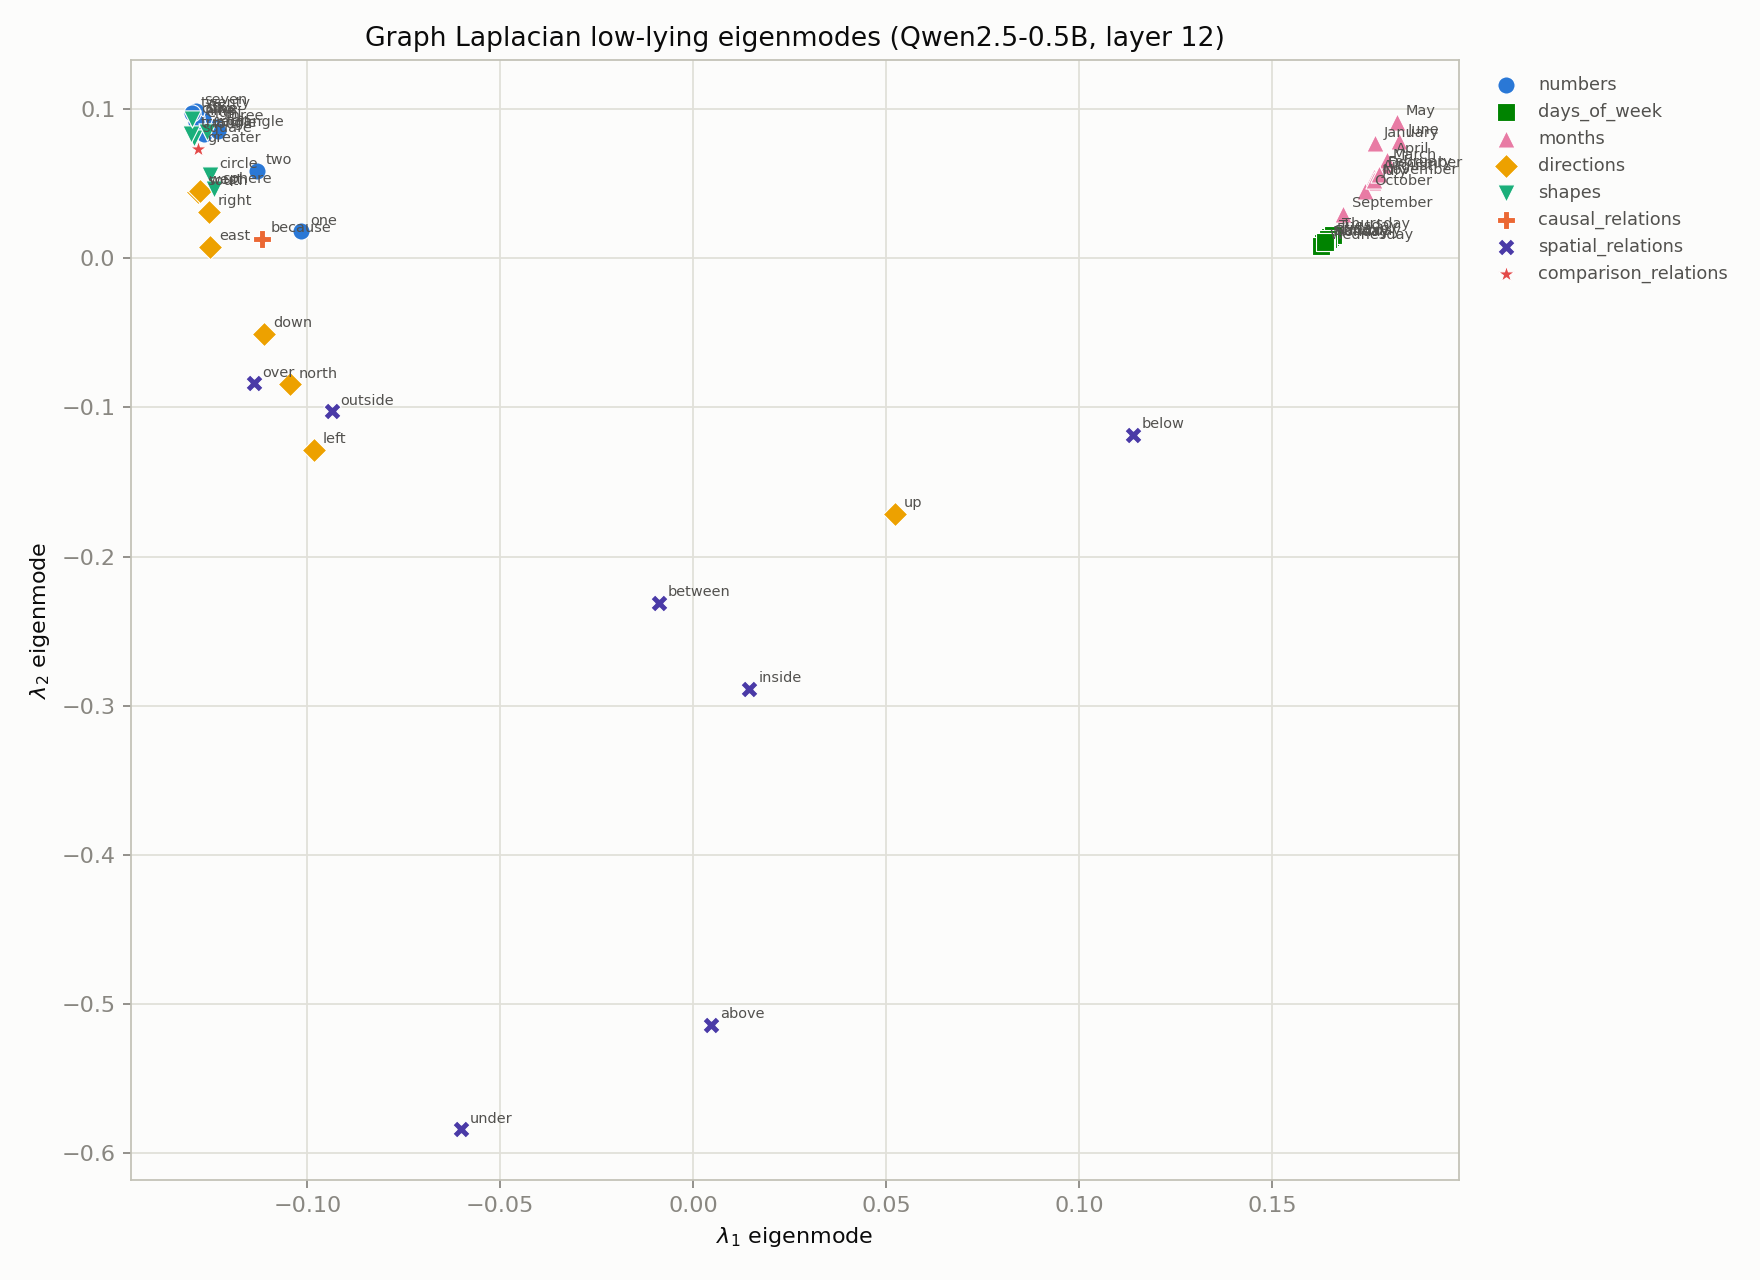
\includegraphics[width=0.85\textwidth]{figures/eigenmodes_2d.png}
  \caption{Qwen2.5-0.5B, layer 12: low-lying Laplacian eigenmodes for 53
  single-token probes. Marker shape and color both encode category.}
  \label{fig:qwen2d}
\end{figure}

The $g{=}0$ control (Figure~\ref{fig:spectrum}) confirms this is a real,
above-noise effect: the structured probe set's spectrum shows a sharp jump
after the second eigenvalue (gap ratio $\lambda_3/\lambda_2 \approx 8.0$),
while randomized single-token vocabulary strings, run through the identical
pipeline, produce a much smoother, more gradual spectrum (gap ratio
$\approx 2.1$).

\begin{figure}[H]
  \centering
  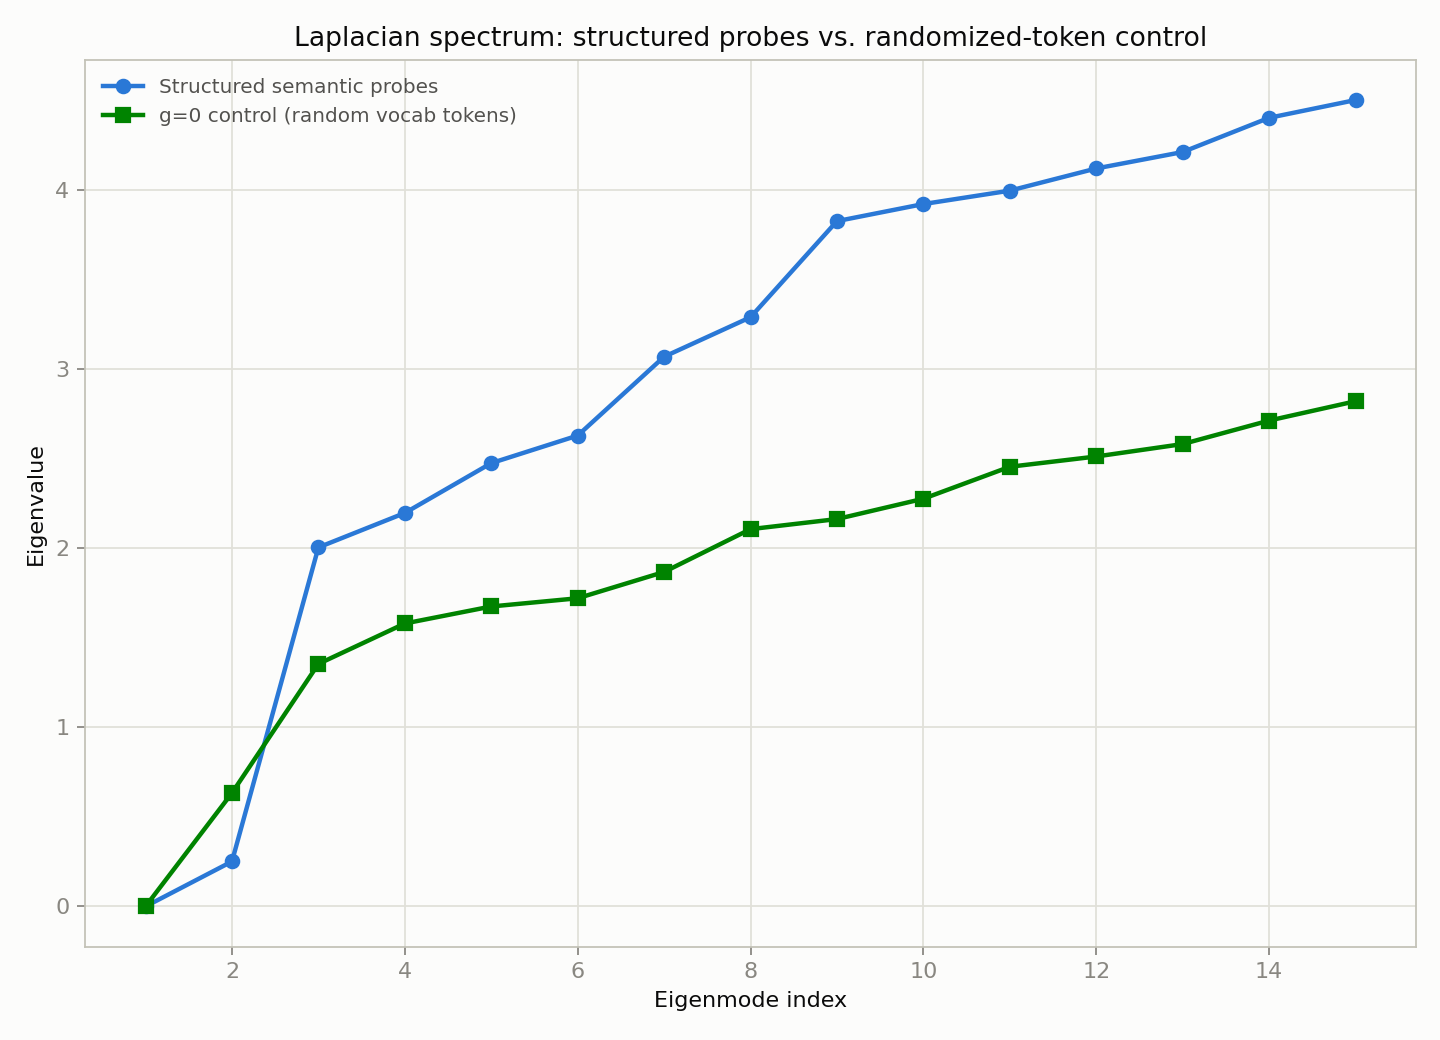
\includegraphics[width=0.75\textwidth]{figures/spectrum_comparison.png}
  \caption{Laplacian eigenvalue spectrum: structured semantic probes vs.\ the
  $g{=}0$ randomized-token control. The structured set shows a much sharper
  spectral gap.}
  \label{fig:spectrum}
\end{figure}

\subsection{Mistral-7B-v0.1: the same separation, much sharper}

Repeating the pipeline on Mistral-7B-v0.1 (layer 16, 4-bit) produced a
striking result: the graph split into exactly two \emph{fully disconnected}
components after negative-weight clipping. One component contained every
calendar/cyclic probe (all 7 days-of-week and all 12 months, 19 tokens); the
other contained every remaining probe (numbers, directions, shapes, causal,
spatial, and comparison relations, 44 tokens). There were zero
positive-similarity edges between the two groups, a sharper separation than
the small model showed.

\begin{figure}[H]
  \centering
  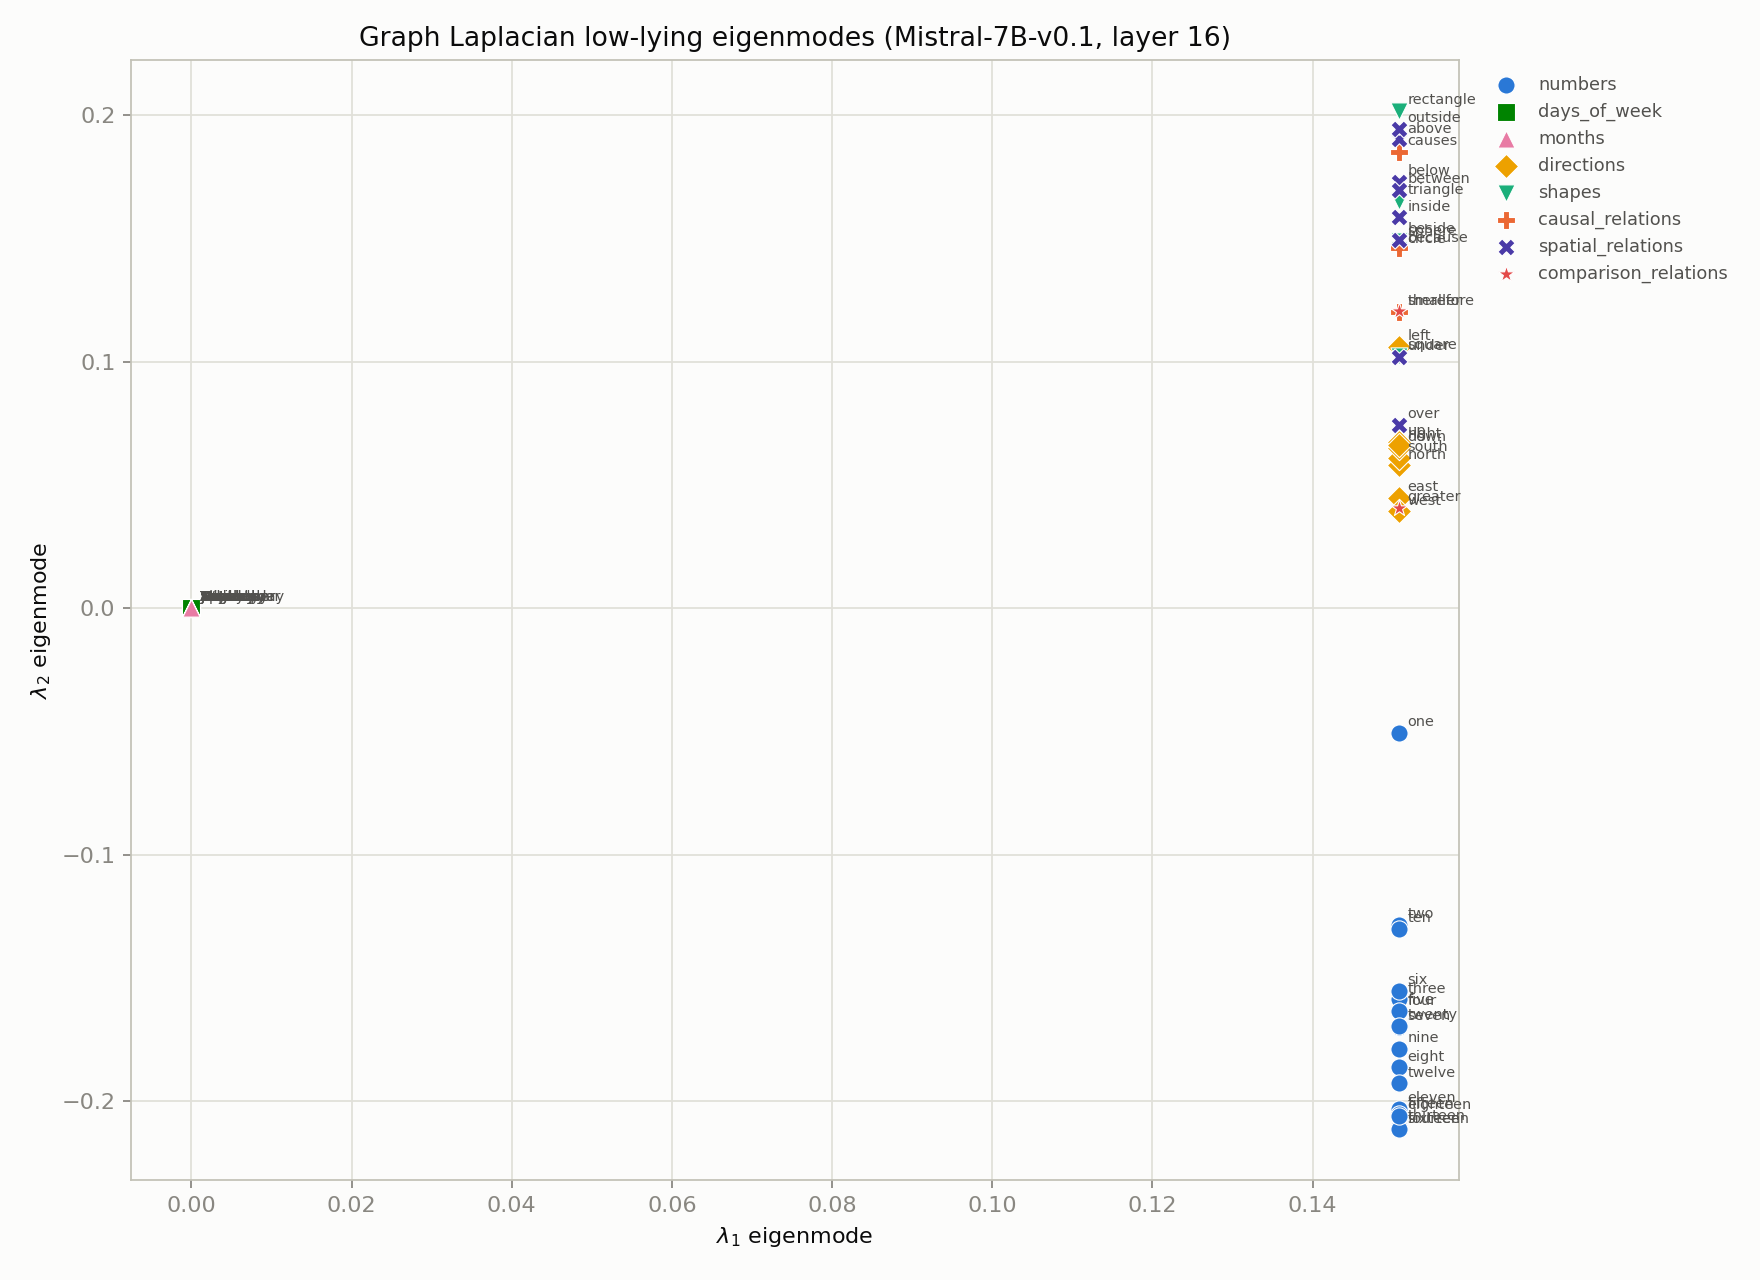
\includegraphics[width=0.85\textwidth]{figures/eigenmodes_mistral_2d.png}
  \caption{Mistral-7B-v0.1, layer 16: the calendar/cyclic island (right) is
  completely disconnected from every other probe category (left).}
  \label{fig:mistral2d}
\end{figure}

Isolating that 19-token calendar island and diagonalizing it on its own
(Figure~\ref{fig:mistralcal}) did \emph{not} reveal a clean circle within it:
the 7 days-of-week collapsed into indistinguishable, overlapping points, while
the 12 months traced a single smooth hump along one axis (peak near May,
trough near December) with almost no variation along the other axis, a 1D
pattern, not a 2D loop.

\begin{figure}[H]
  \centering
  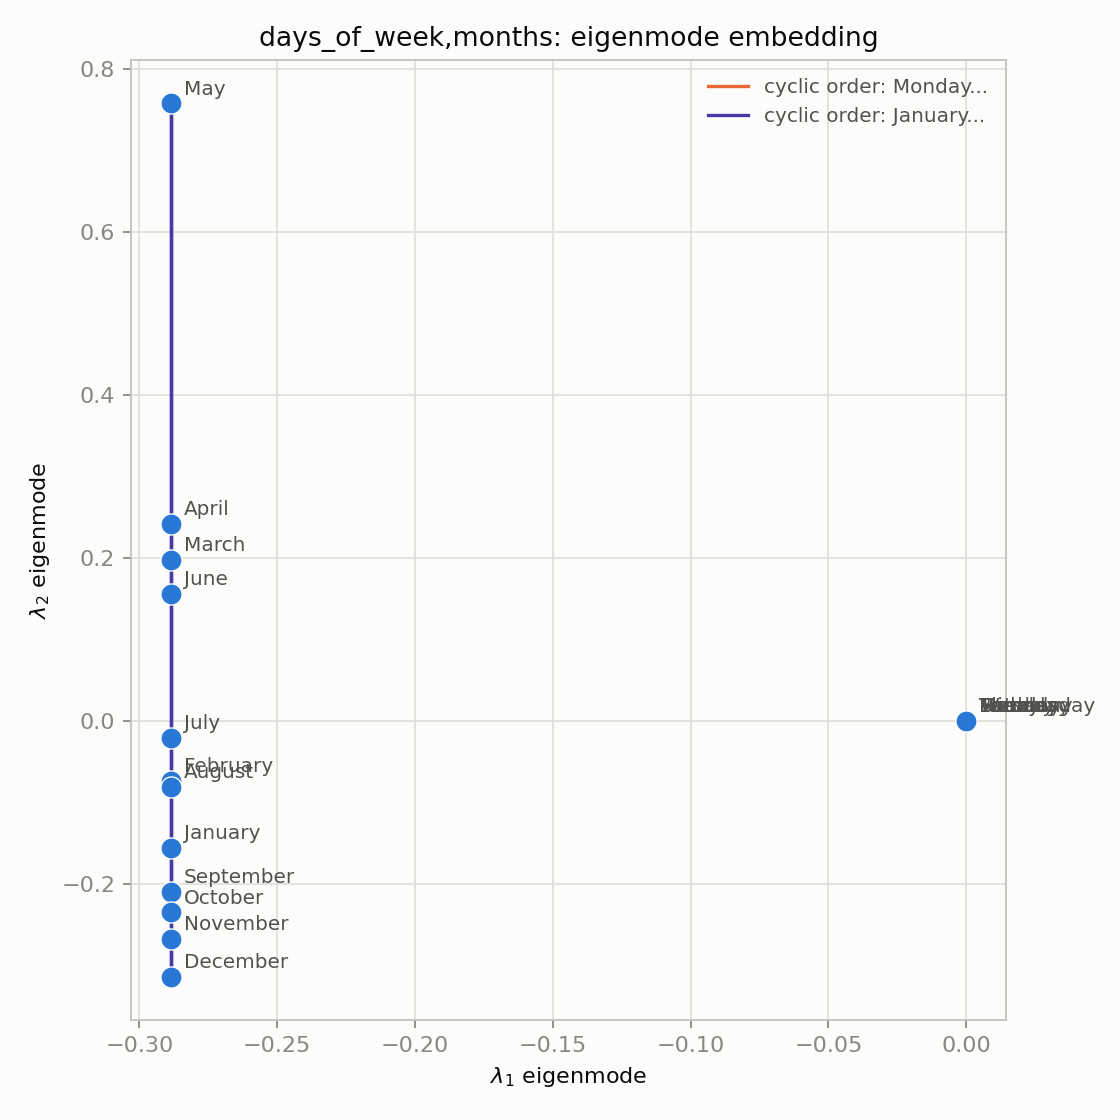
\includegraphics[width=0.7\textwidth]{figures/days_months_mistral.png}
  \caption{Mistral-7B-v0.1: the isolated calendar component, diagonalized on
  its own. Days-of-week (right, overlapping) show no internal structure;
  months (left) show a 1D hump, not a 2D circle.}
  \label{fig:mistralcal}
\end{figure}

\subsection{Scaling to 500 tokens: the calendar cluster holds, and a broader pattern emerges}
\label{sec:scale500result}

Figures~\ref{fig:qwen500} and~\ref{fig:mistral500} show the low-lying
eigenmode embedding for all 25 categories at the full 500-token scale. Two
findings replicate directly from the 77-token experiments: days-of-week and
months still cluster tightly together in both models, distinct from the rest
of the probe set, and the categorical separation is again visibly sharper in
Mistral-7B than in Qwen2.5-0.5B.

\begin{figure}[H]
  \centering
  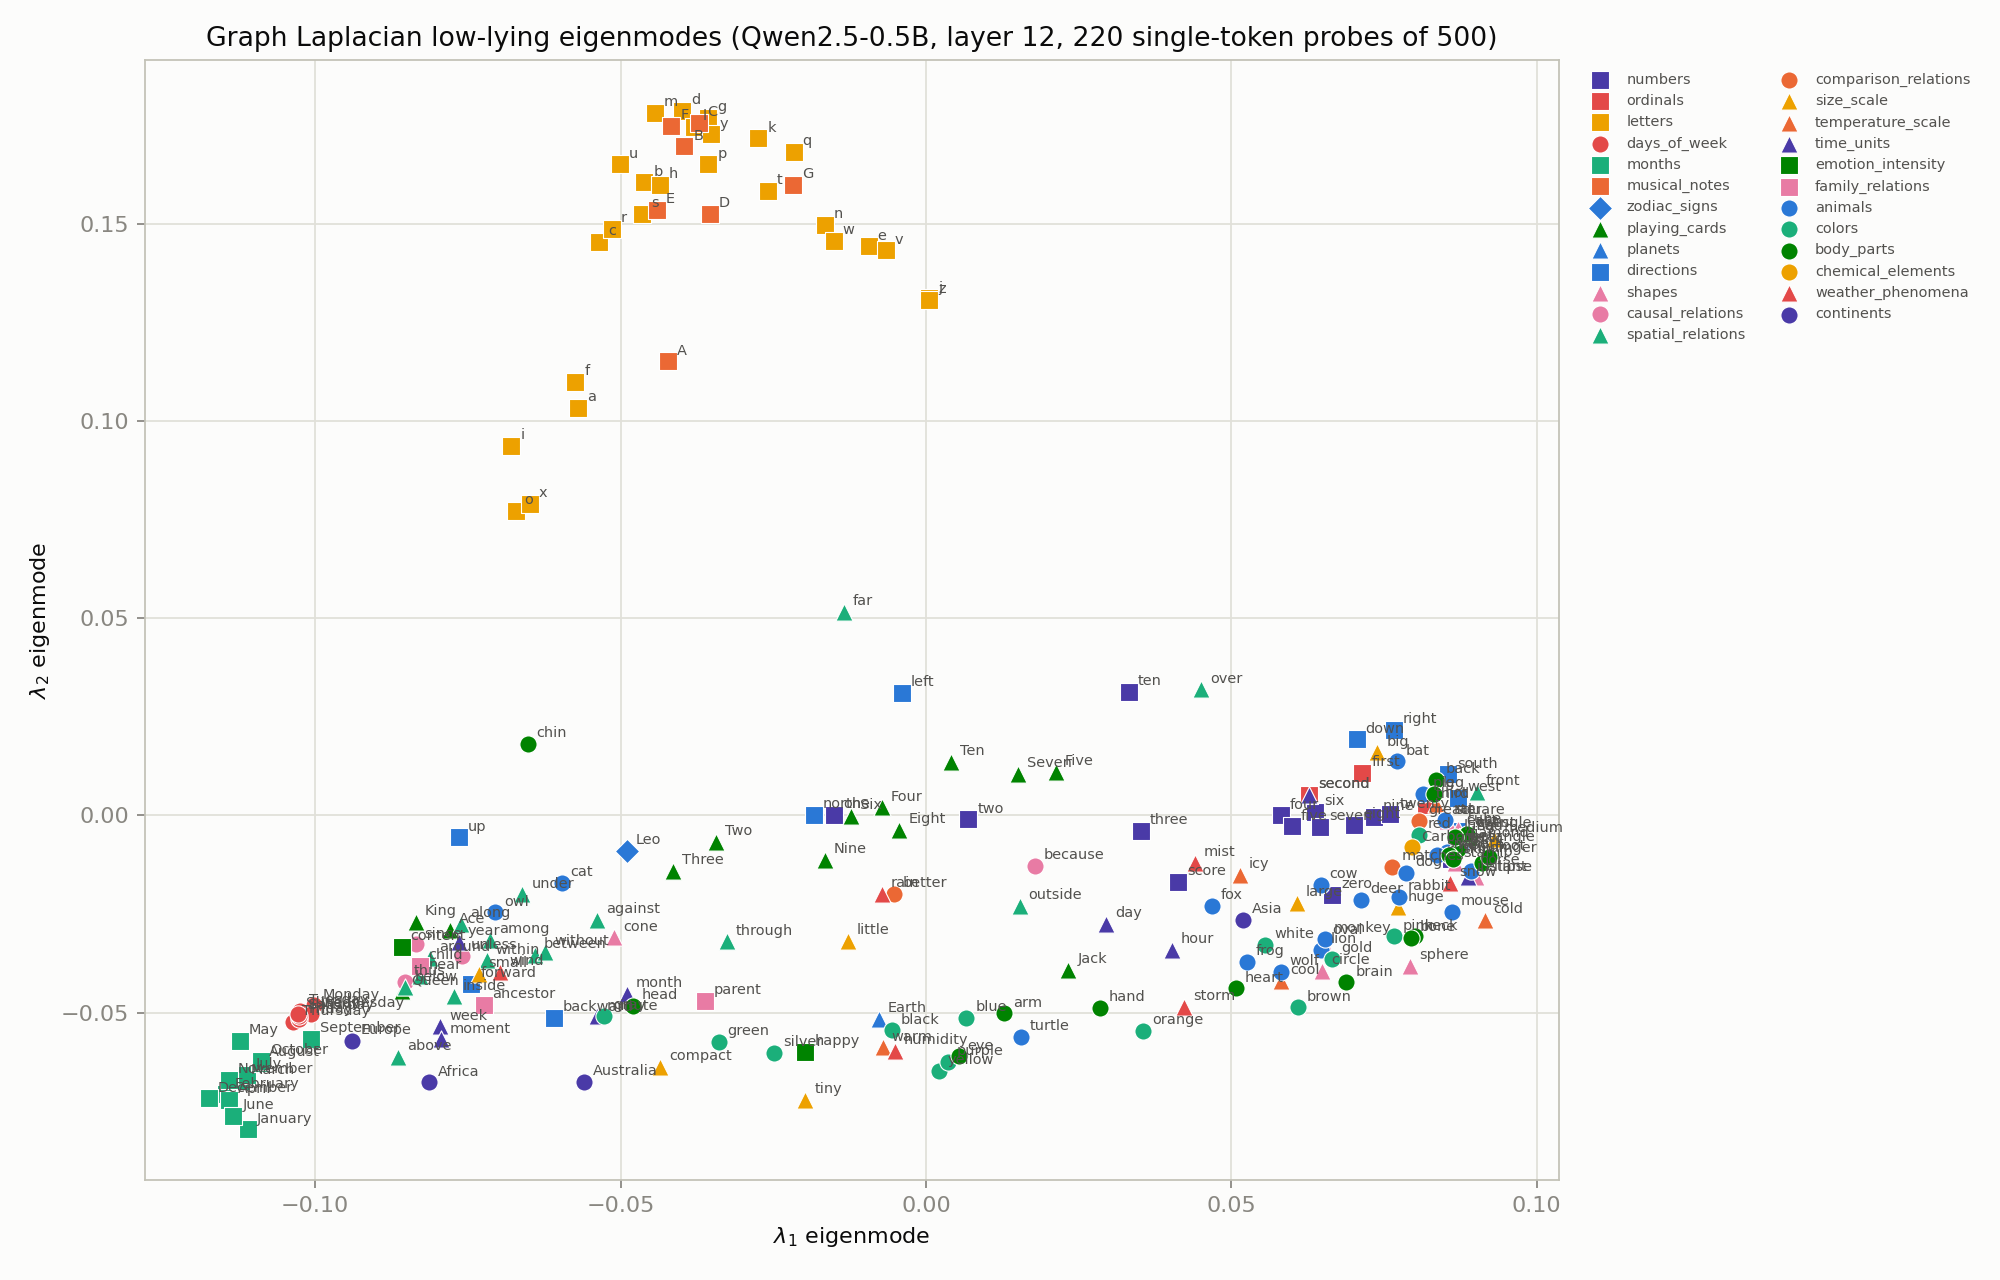
\includegraphics[width=\textwidth]{figures/eigenmodes_500_2d.png}
  \caption{Qwen2.5-0.5B, layer 12, 500-token probe set (220 single-token
  probes shown). Days-of-week and months again cluster tightly (bottom
  left); letters trace a visible arc (top).}
  \label{fig:qwen500}
\end{figure}

\begin{figure}[H]
  \centering
  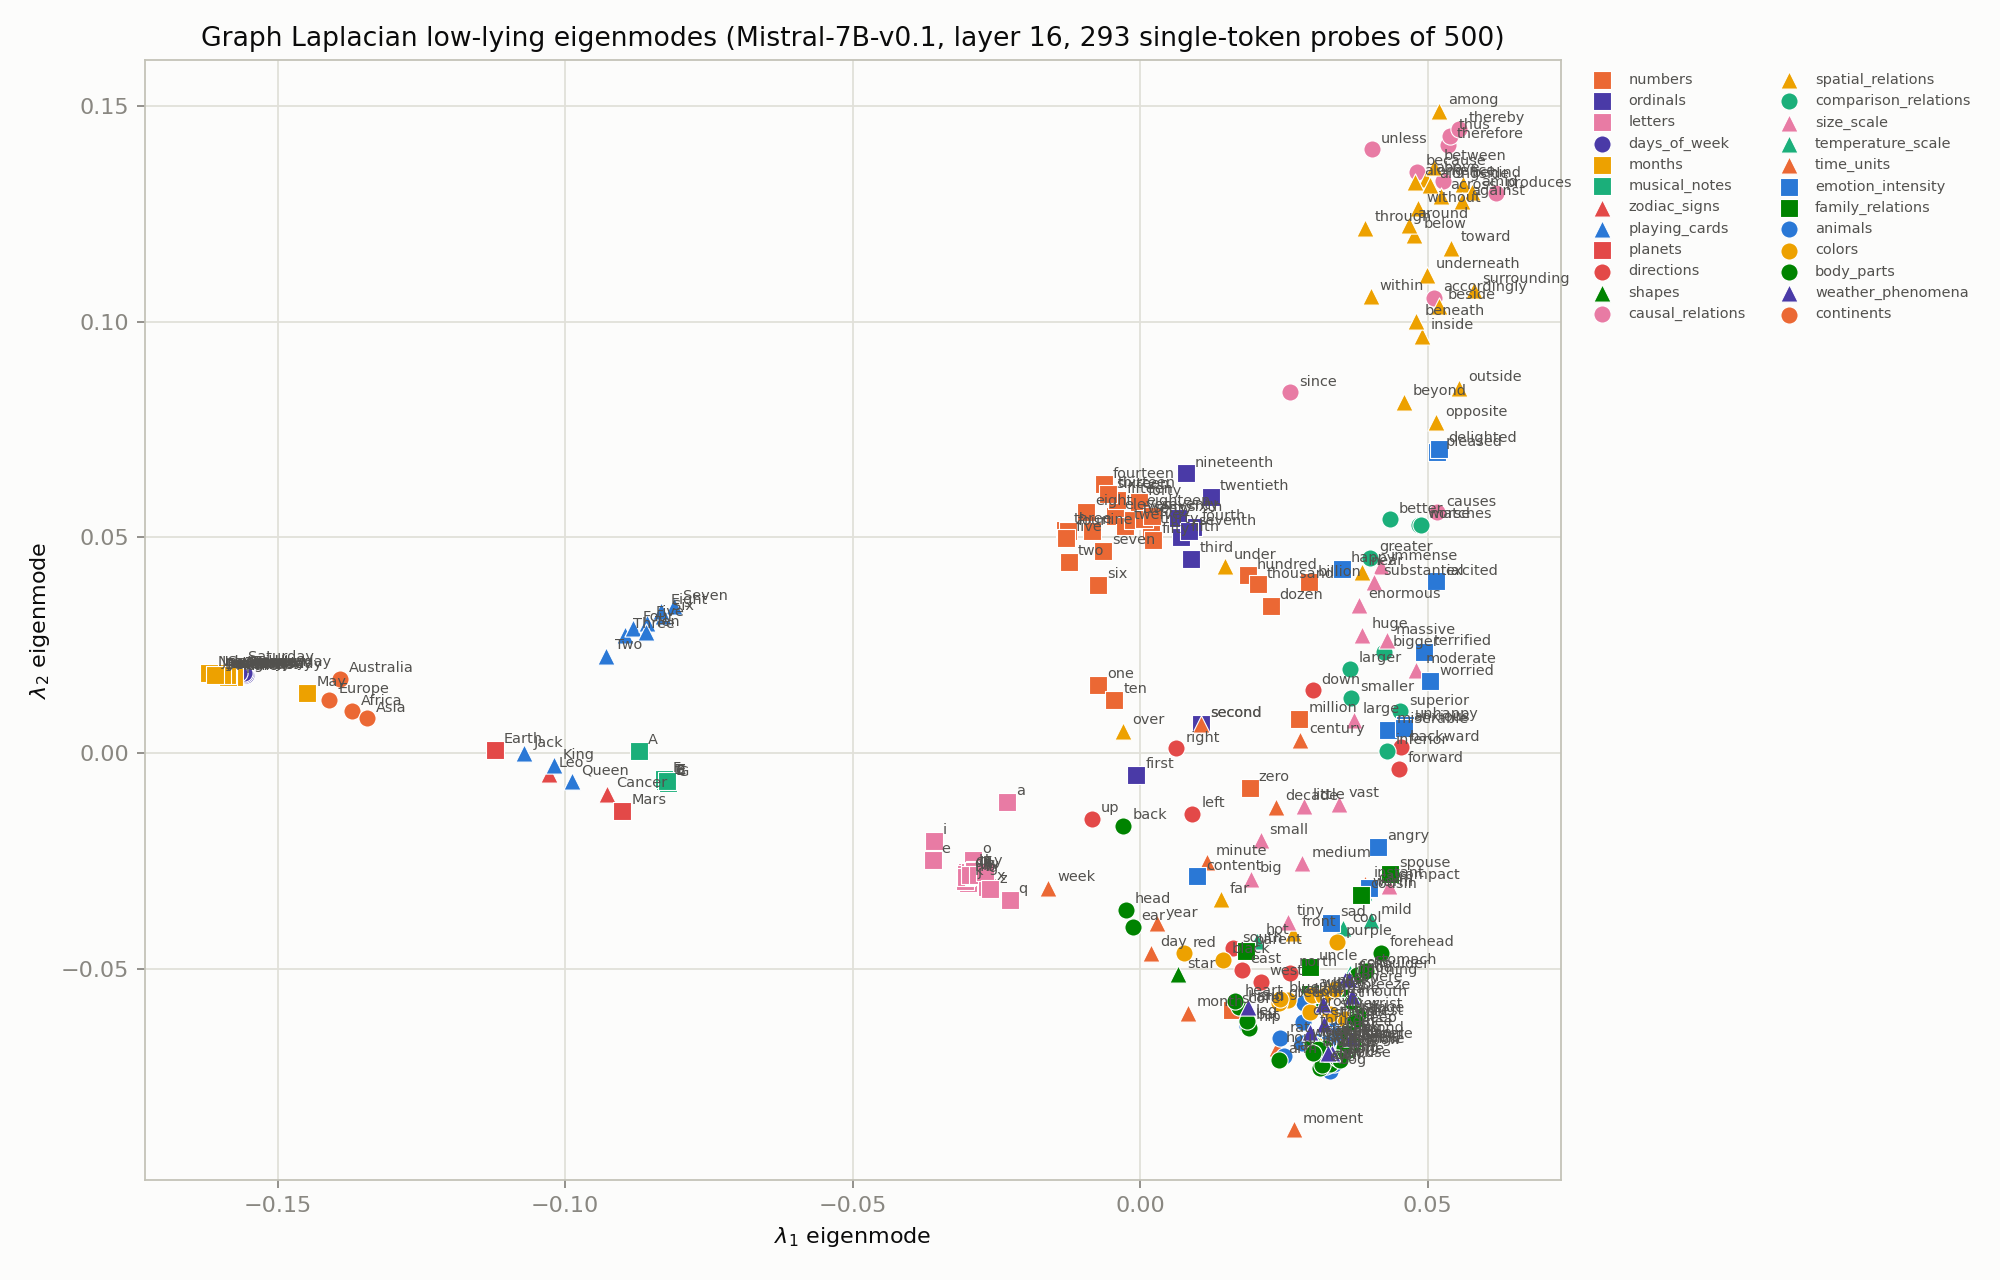
\includegraphics[width=\textwidth]{figures/eigenmodes_mistral_500_2d.png}
  \caption{Mistral-7B-v0.1, layer 16, 500-token probe set (293 single-token
  probes shown). The calendar cluster (far left) is joined by continents
  nearby; playing-card ranks form their own island, separate from ordinary
  cardinal numbers despite sharing the same words; the remaining
  no-expected-structure categories (animals, colors, body parts, emotions,
  weather, directions) collapse into one dense, largely undifferentiated
  region (bottom right).}
  \label{fig:mistral500}
\end{figure}

The larger, more varied category set surfaces a pattern the original 8
categories could not have shown: the categories that separate cleanly are
not specifically \emph{cyclic/temporal} ones, but \emph{small, closed,
enumerable named sets} more generally. In Mistral-7B, days-of-week, months,
continents, zodiac signs, playing-card ranks, and planets each form their
own distinguishable region, none of which are all cyclic (continents and
planets have no natural cyclic order at all), but all of which name one of a
small, fixed, exhaustively enumerable list. By contrast, the categories we
deliberately chose to have no expected relational structure at all (animals,
colors, body parts, weather phenomena, emotion intensity) collapse into one
large, largely undifferentiated region, a second, richer negative control
alongside the $g{=}0$ random-vocabulary control, and one that emerged from
the data rather than being designed in. A particularly sharp illustration:
playing-card rank words (\emph{Two}, \emph{Seven}, \emph{King}, \ldots)
occupy a visibly different region from the ordinary cardinal numbers
(\emph{two}, \emph{seven}, \ldots) despite the literal word overlap for the
numeric ranks, suggesting the model's representation at this position is
organized around which closed set a token names, not the token's surface
form or numeric value alone.

\subsection{Template-based PCA: months show a real loop, days do not}

Switching from bare-word probing to in-context arithmetic prompts (\emph{``The
day/month after X is''}) and ordinary PCA produced a qualitatively different,
partially positive result. A sanity check (Table~\ref{tab:tasksanity})
confirmed Mistral-7B solves this task correctly for 19 of 20 prompts (missing
only the December$\to$January wraparound).

\label{sec:tasksanity}
\begin{table}[H]
  \centering
  \begin{tabular}{lc}
    \toprule
    Task & Accuracy \\
    \midrule
    Day-after (7 prompts)   & 7/7 \\
    Month-after (12 prompts) & 11/12 (December$\to$``always'', not January) \\
    \bottomrule
  \end{tabular}
  \caption{Sanity check: does the model actually solve the arithmetic task
  used to elicit the probed representations?}
  \label{tab:tasksanity}
\end{table}

Months (Figure~\ref{fig:monthspca}) traced a recognizable, mostly
non-self-crossing loop in calendar order across the top two principal
components, with one small local crossing near March--April--May. Days of the
week (Figure~\ref{fig:dayspca}), under the identical method, produced a
messy, repeatedly self-crossing path with no discernible circular order.

\begin{figure}[H]
  \centering
  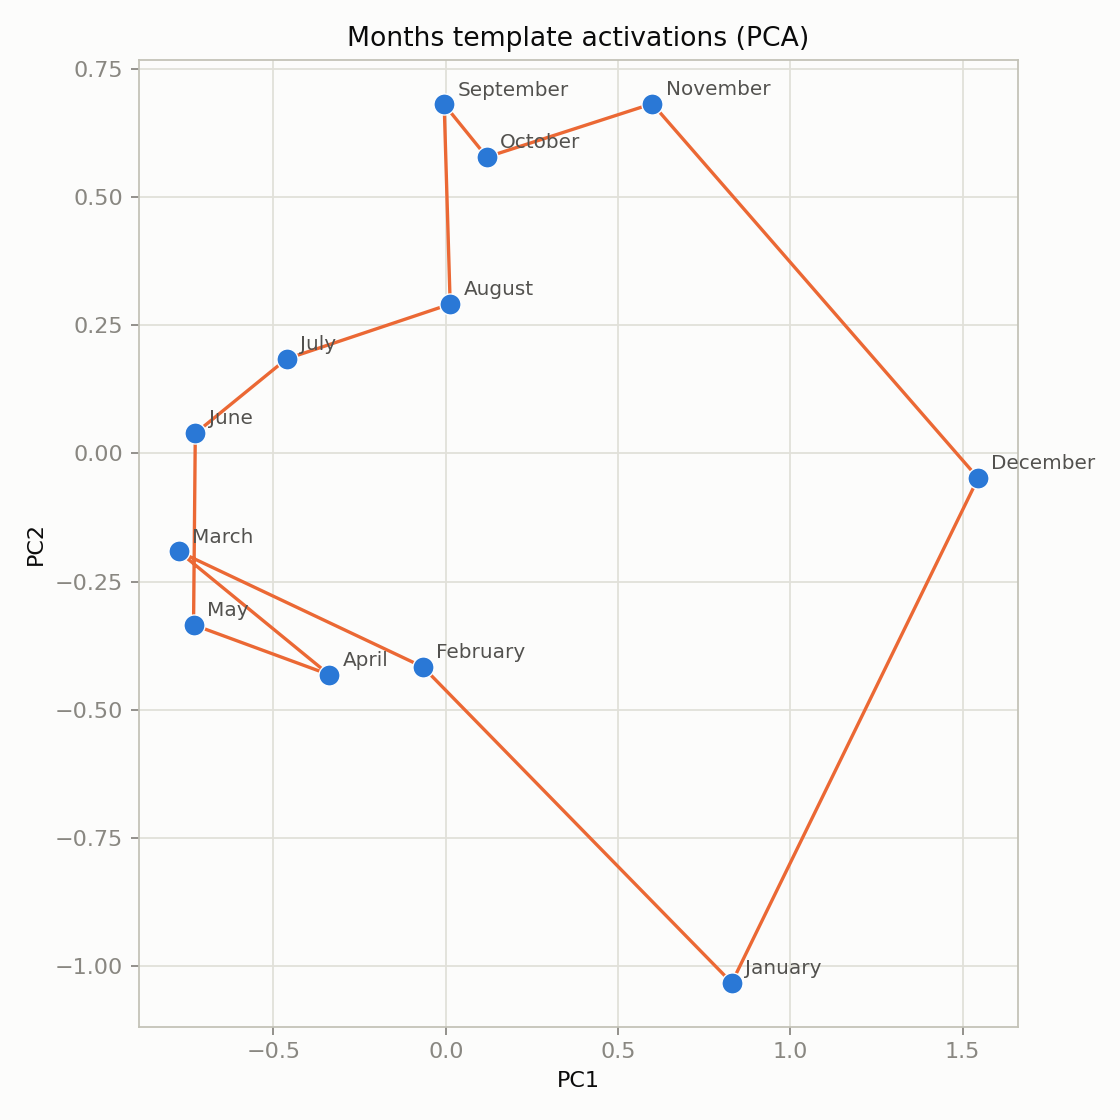
\includegraphics[width=0.7\textwidth]{figures/months_template_pca.png}
  \caption{Months, template-elicited activations, top-2 PCA: a mostly clean
  loop in calendar order.}
  \label{fig:monthspca}
\end{figure}

\begin{figure}[H]
  \centering
  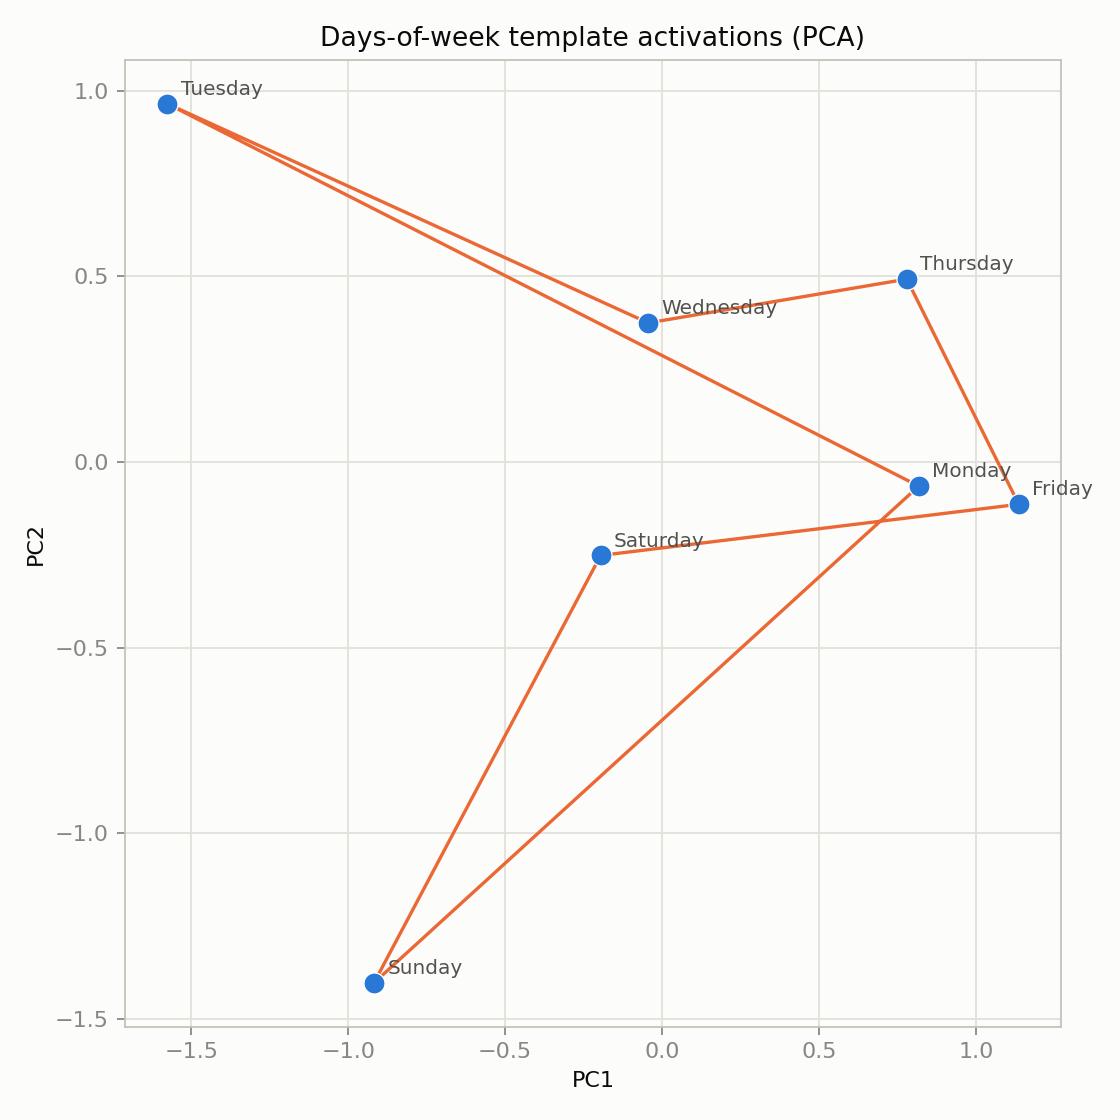
\includegraphics[width=0.7\textwidth]{figures/days_template_pca.png}
  \caption{Days of week, identical method: a self-crossing path, not a loop.}
  \label{fig:dayspca}
\end{figure}

\subsection{Causal activation patching, attempt 1: a null result, with a diagnosis}

The patching experiment (last-token hidden state at layer 16, base prompt
patched with a donor prompt's activation) produced \textbf{zero} effect: the
model's top-1 prediction after patching was identical, in every single
(base, donor) pair tested (7 for days, 12 for months), to the prediction the
\emph{unpatched} base prompt would have produced. The random-direction control
also produced no shift toward the donor's expected answer, for the same
reason: neither intervention changed the output at all.

We do not read this as evidence against a causal role for the patched
subspace. The prompts still contained the literal day/month name as plain
text at an earlier position (e.g., \emph{``The day after \textbf{Monday} is''}).
Patching only the final token's hidden state does not prevent later attention
layers from simply re-reading the day name directly from its own token
position in the prompt: the intervention we implemented could be
circumvented by the model without ever using the patched representation.
This is a known pitfall in activation patching: a clean causal-tracing
experiment requires patching at the subject-token position itself (here, the
day/month name), not merely a downstream summary position, so that the
information cannot be recovered by re-attending to the original input.

\subsection{Causal activation patching, attempt 2: a clean, strongly positive result}
\label{sec:causalresult}

Redoing the intervention at the subject-token position (\S\ref{sec:causaltrace2},
swept across all 32 layers) produced exactly the kind of result a real causal
effect should look like (Figure~\ref{fig:causaltrace}). For both categories:

\begin{itemize}
  \item \textbf{Real donor patches work almost perfectly through the early-to-mid
        layers.} Days-of-week: 100\% patch accuracy from layer 0 through
        layer 19. Months: 83--100\% accuracy from layer 0 through layer 16.
        Swapping in a different day/month's representation at this one token
        position, at these layers, is sufficient to flip the model's final
        answer to match the donor, exactly as if the input word itself had
        been changed.
  \item \textbf{The effect collapses sharply past a well-defined depth.} Days:
        accuracy drops to 29\% at layer 20 and 0\% from layer 21 on. Months:
        it drops to 8\% at layer 17 and 0\% from layer 18 on. This is a
        genuine localization result, not a gradual fade, consistent with
        the model reading the subject identity out of this position by a
        certain depth and no longer needing to re-derive it from there in
        later layers.
  \item \textbf{The random-direction control stays at exactly 0.00 at every
        single layer, for both categories.} Perturbing the residual stream by
        the same magnitude in a random direction never once produces the
        donor's expected answer. The effect above is specific to the donor's
        real representation, not an artifact of disturbing the activation by
        some amount.
\end{itemize}

\begin{figure}[H]
  \centering
  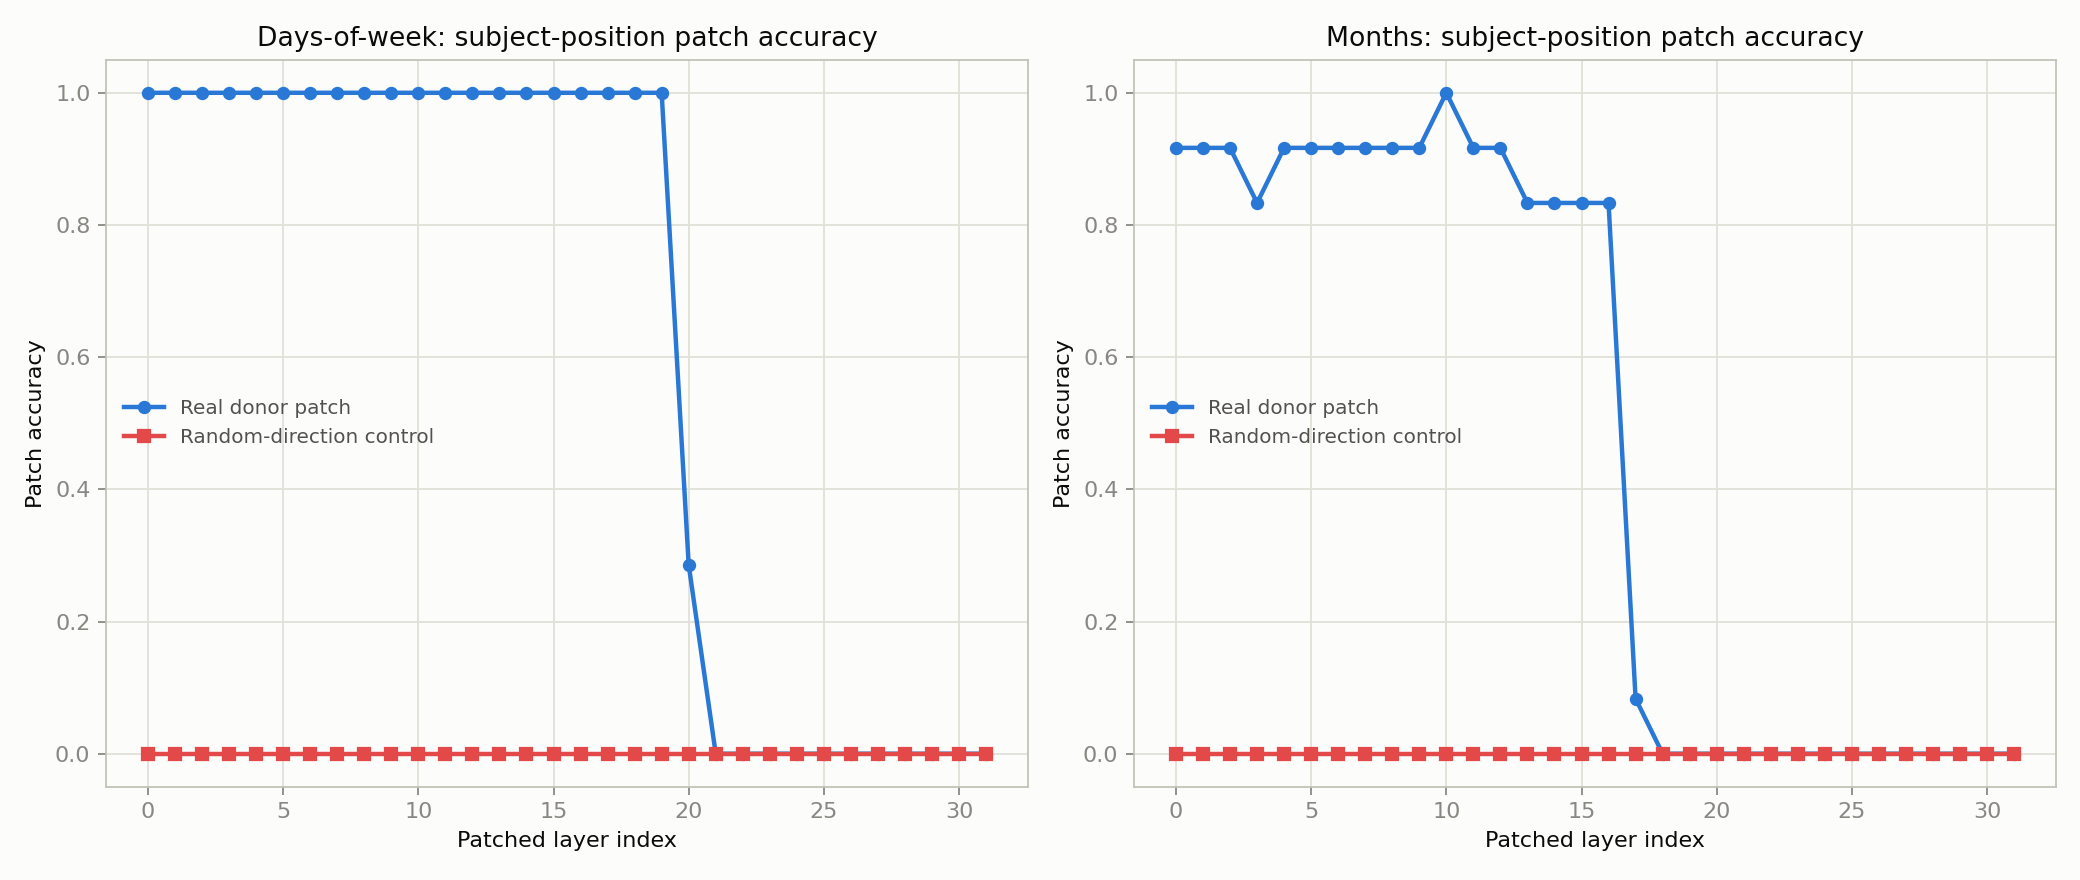
\includegraphics[width=\textwidth]{figures/causal_trace.png}
  \caption{Causal-tracing layer sweep on Mistral-7B-v0.1: patch accuracy vs.\
  the layer at which the subject-token position is overwritten with a
  donor's representation. Real patches (blue) work almost perfectly through
  early-to-mid layers and collapse sharply past a well-defined depth; the
  random-direction control (red) never once succeeds, at any layer.}
  \label{fig:causaltrace}
\end{figure}

This is a real, positive causal result: the day/month identity encoded at the
subject-token position is not merely correlational structure sitting in
activation space: the model actually reads it from that position and uses
it to compute its answer, and an experimenter who swaps it out gets to control
that answer. It does \emph{not}, on its own, prove the stronger geometric
claim that this identity is encoded specifically as a point on a 2D circle
(as opposed to some other, non-circular high-dimensional code that happens to
support this arithmetic). Confirming that would require patching specifically
along the rotation direction of the loop found in \S\ref{sec:tasksanity}'s PCA
(for months, where that loop was cleanest) rather than swapping in a whole
different item's representation, and is the natural next experiment.

\subsection{Causal activation patching, attempt 3: a clean loop that is not a causal code}
\label{sec:rotationresult}

Figure~\ref{fig:rotationpca} shows the position-4, layer-12 PCA embedding used
for this test. Months trace the cleanest 2D loop found anywhere in this
project: a near-convex, non-self-crossing polygon that visits every month in
exact calendar order (May $\to$ June $\to \cdots \to$ April $\to$ back to
May). Days-of-week, consistent with every earlier attempt, does not: Tuesday,
Wednesday, Thursday, Saturday, Friday, Sunday, Monday form a path with a sharp
spike at Saturday, not a clean loop.

\begin{figure}[H]
  \centering
  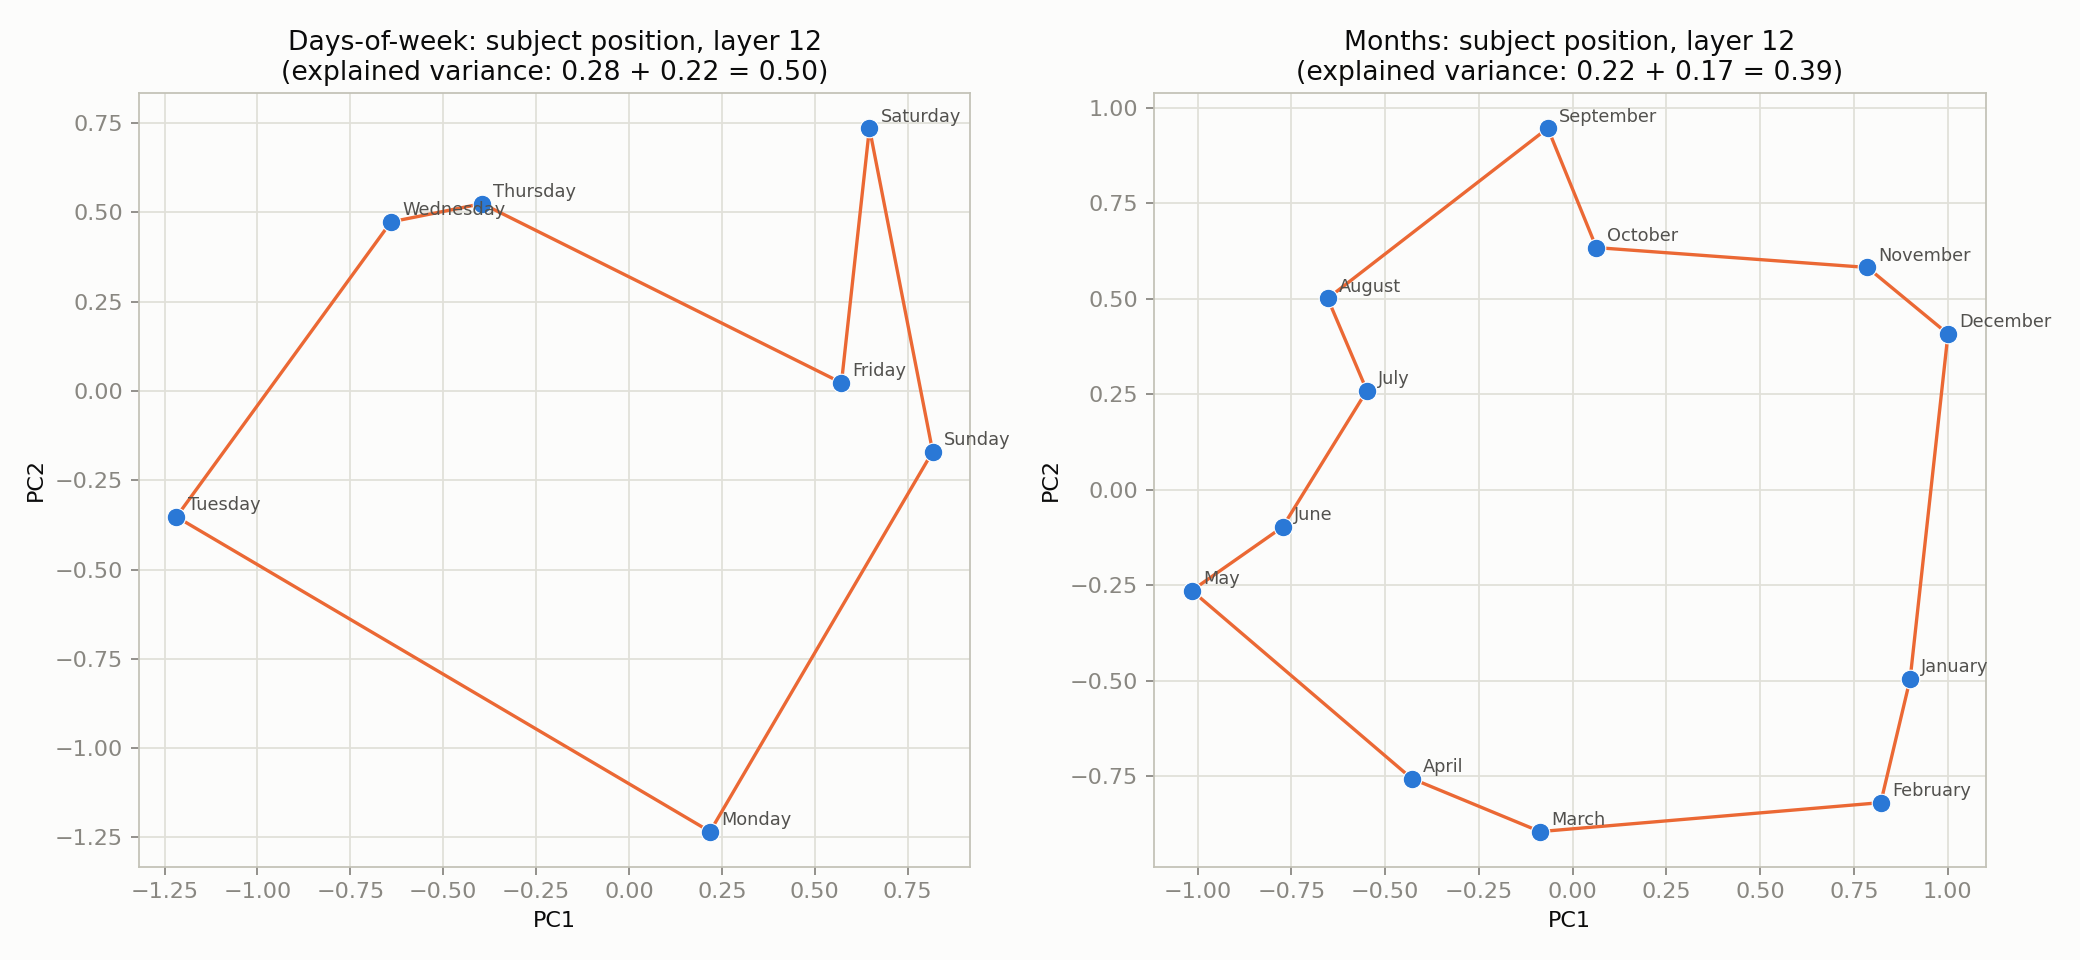
\includegraphics[width=\textwidth]{figures/rotation_pca.png}
  \caption{Subject-token-position PCA at layer 12. Months (right) trace an
  almost perfectly convex loop in calendar order; days-of-week (left) does
  not. Only 39\% (months) and 50\% (days) of the position's variance is
  captured by these two components.}
  \label{fig:rotationpca}
\end{figure}

Despite that clean loop, the rotation experiment is a clear, symmetric null
result:

\begin{itemize}
  \item \textbf{Real donor patches at this layer}: 35/35 (100\%) for days,
        49/60 (82\%) for months, consistent with attempt 2's layer sweep at
        layer 12.
  \item \textbf{Synthetic rotation, correct calendar-consistent angle}: 3/35
        (9\%) for days, 0/60 (0\%) for months.
  \item \textbf{Synthetic rotation, deliberately wrong off-lattice angle}:
        3/35 (9\%) for days, 0/60 (0\%) for months, statistically
        indistinguishable from the ``correct'' angle. Line-by-line, the two
        conditions frequently produce the exact same output token for the
        exact same base item, meaning whether the rotation angle matched a
        real calendar offset made no detectable difference at all: both
        conditions mostly degenerate to filler tokens (\emph{the}, \emph{a},
        \emph{always}) rather than any coherent month or day name.
\end{itemize}

The top-2 PCA plane at this position explains only 39\% (months) and 50\%
(days) of the variance there. Reconstructing a vector from just those two
components and rotating within them discards enough of the real,
high-dimensional structure that the result is no longer parseable by the
model as \emph{any} coherent day or month, let alone the correct one, and the
correctness of the rotation angle is irrelevant to that failure. The 2D loop
visible in Figure~\ref{fig:rotationpca} is a real, reproducible visual
pattern, and it is not, on the evidence here, the causal code the model
actually uses.

\subsection{Causal activation patching, attempt 4: the full-rank rotation recovers the effect}
\label{sec:highdimresult}

Figure~\ref{fig:rotationsummary} summarizes every patching condition tested
in this paper, at the same layer (12) and subject-token position. The
full-rank rotation generator, fit once across all items via orthogonal
Procrustes, closes almost all of the gap left open by attempt 3:

\begin{itemize}
  \item \textbf{Days-of-week}: full-rank rotation reaches 35/35 (100\%),
        identical to the real donor patch, and far above the 2D rotation's
        3/35 (9\%).
  \item \textbf{Months}: full-rank rotation reaches 51/60 (85\%), matching
        (in fact marginally exceeding) the real donor patch's 49/60 (82\%),
        and far above the 2D rotation's 0/60 (0\%).
  \item \textbf{The fractional-power control collapses}, to 5/35 (14\%) for
        days and 5/60 (8\%) for months, both near the noise floor. Only a
        rotation by a real integer offset works; a rotation by almost the
        same angle, fit with the exact same procedure, does not.
\end{itemize}

\begin{figure}[H]
  \centering
  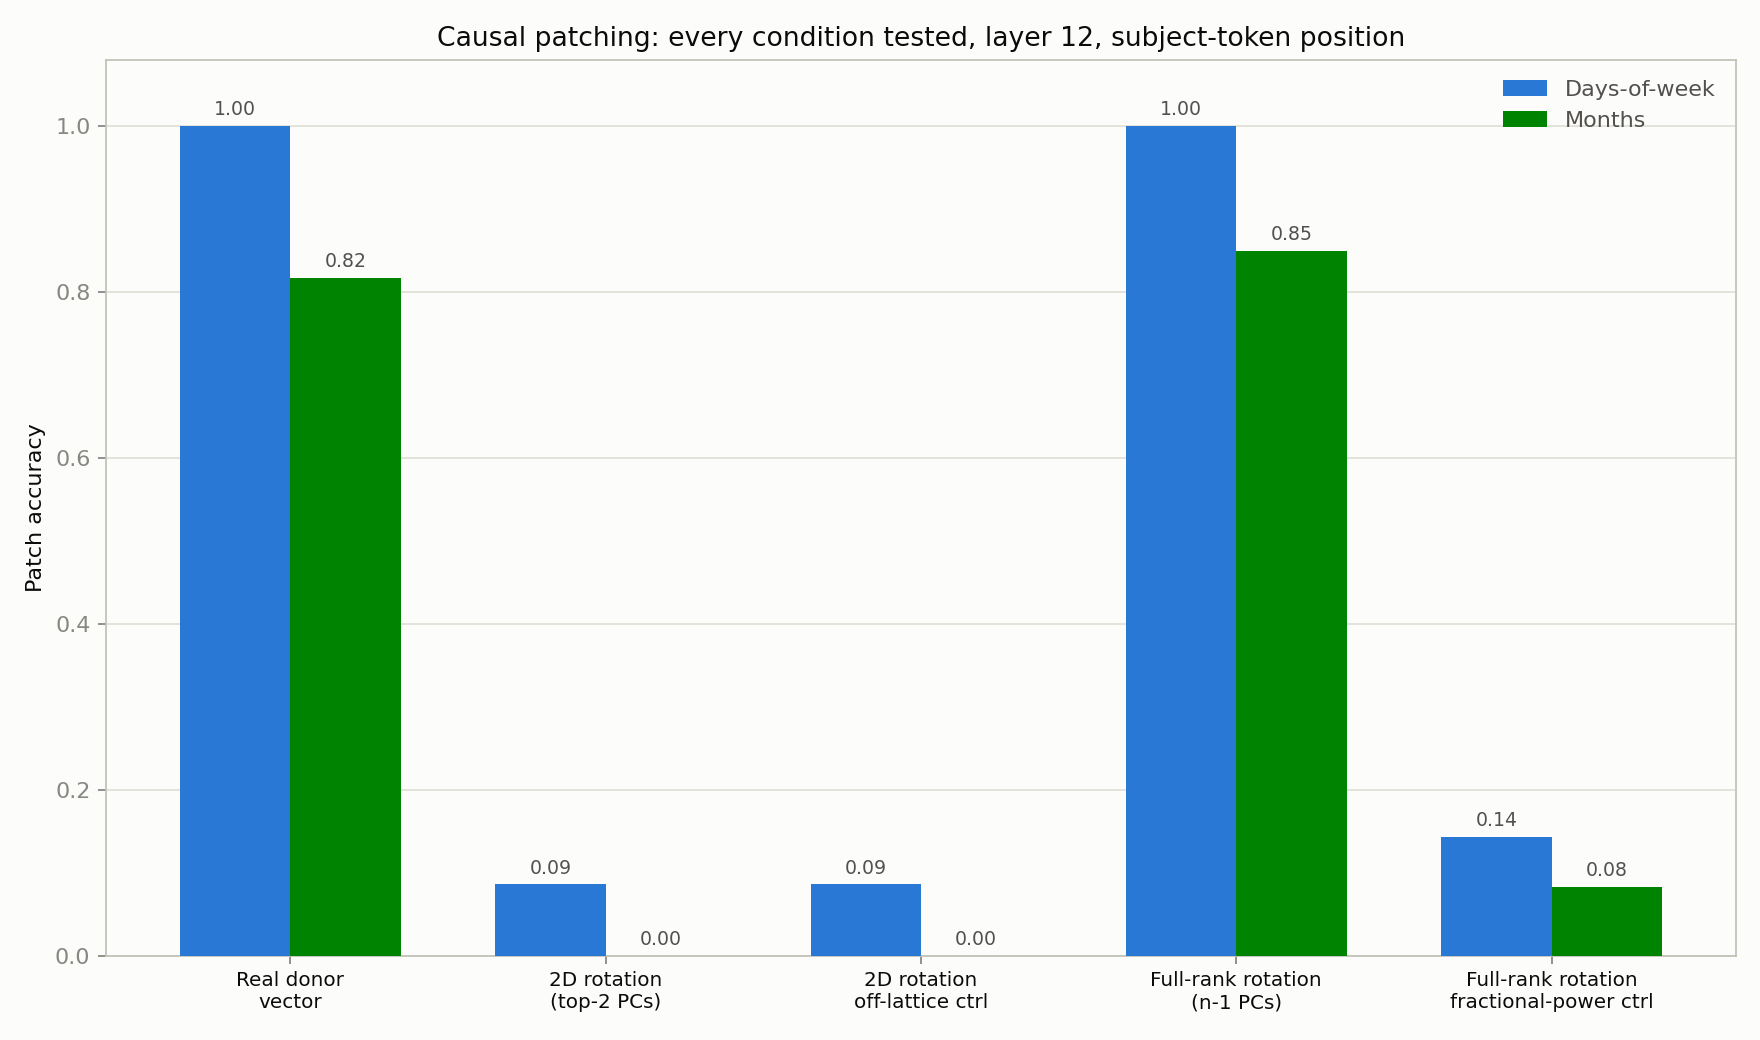
\includegraphics[width=0.9\textwidth]{figures/rotation_summary.png}
  \caption{Every causal-patching condition tested in this paper, side by
  side. The full-rank rotation (4th group) matches the real-donor upper
  bound (1st group) for both categories, while both the 2D rotation (2nd
  group) and the fractional-power control (5th group) collapse toward
  chance.}
  \label{fig:rotationsummary}
\end{figure}

This is a positive result for a genuinely geometric, rotational
interpretation of the causal code, with an important qualification: the
single-rotation-generator Procrustes fit itself has a substantial residual
(26.7\% relative error for days, 23.8\% for months), meaning no single $R$
maps every consecutive pair exactly. Despite that imperfect linear fit, using
$R$'s integer powers as a synthetic intervention still reproduces the full
causal effect, while a small, deliberate deviation in the exponent destroys
it almost entirely. The model's readout at this position appears to care
about approximately which direction, relative to a consistent rotational
structure, the patched vector points, rather than requiring pixel-perfect
fidelity to a real example's activation. That is a meaningfully stronger and
more precise finding than either extreme considered earlier: not the naive
``it's a 2D circle you can see in a PCA plot'' (attempt 3 rules that out),
and not merely ``some opaque high-dimensional code is swappable'' (attempt 2
established that much, but no more); rather, a single consistent rotation
operator, spanning the full space these items occupy, is both necessary
(the fractional-power control fails) and sufficient (no real donor vector is
required) to reproduce the model's behavior.

\subsection{Generalization: partial, and explained by subject-name token length}
\label{sec:generalizeresult}

Figure~\ref{fig:generalization} shows real-donor and full-rank-rotation
accuracy for all five categories tested. The result is a genuine mixed
finding, not a clean replication and not a clean failure:

\begin{itemize}
  \item \textbf{Playing-card ranks generalize well}: 82\% real-donor, 73\%
        full-rank rotation, close to the days/months level and far above the
        other two new categories.
  \item \textbf{Zodiac signs and planets generalize weakly}: 42\%/33\% and
        33\%/17\% respectively, both well below days/months and playing
        cards.
\end{itemize}

\begin{figure}[H]
  \centering
  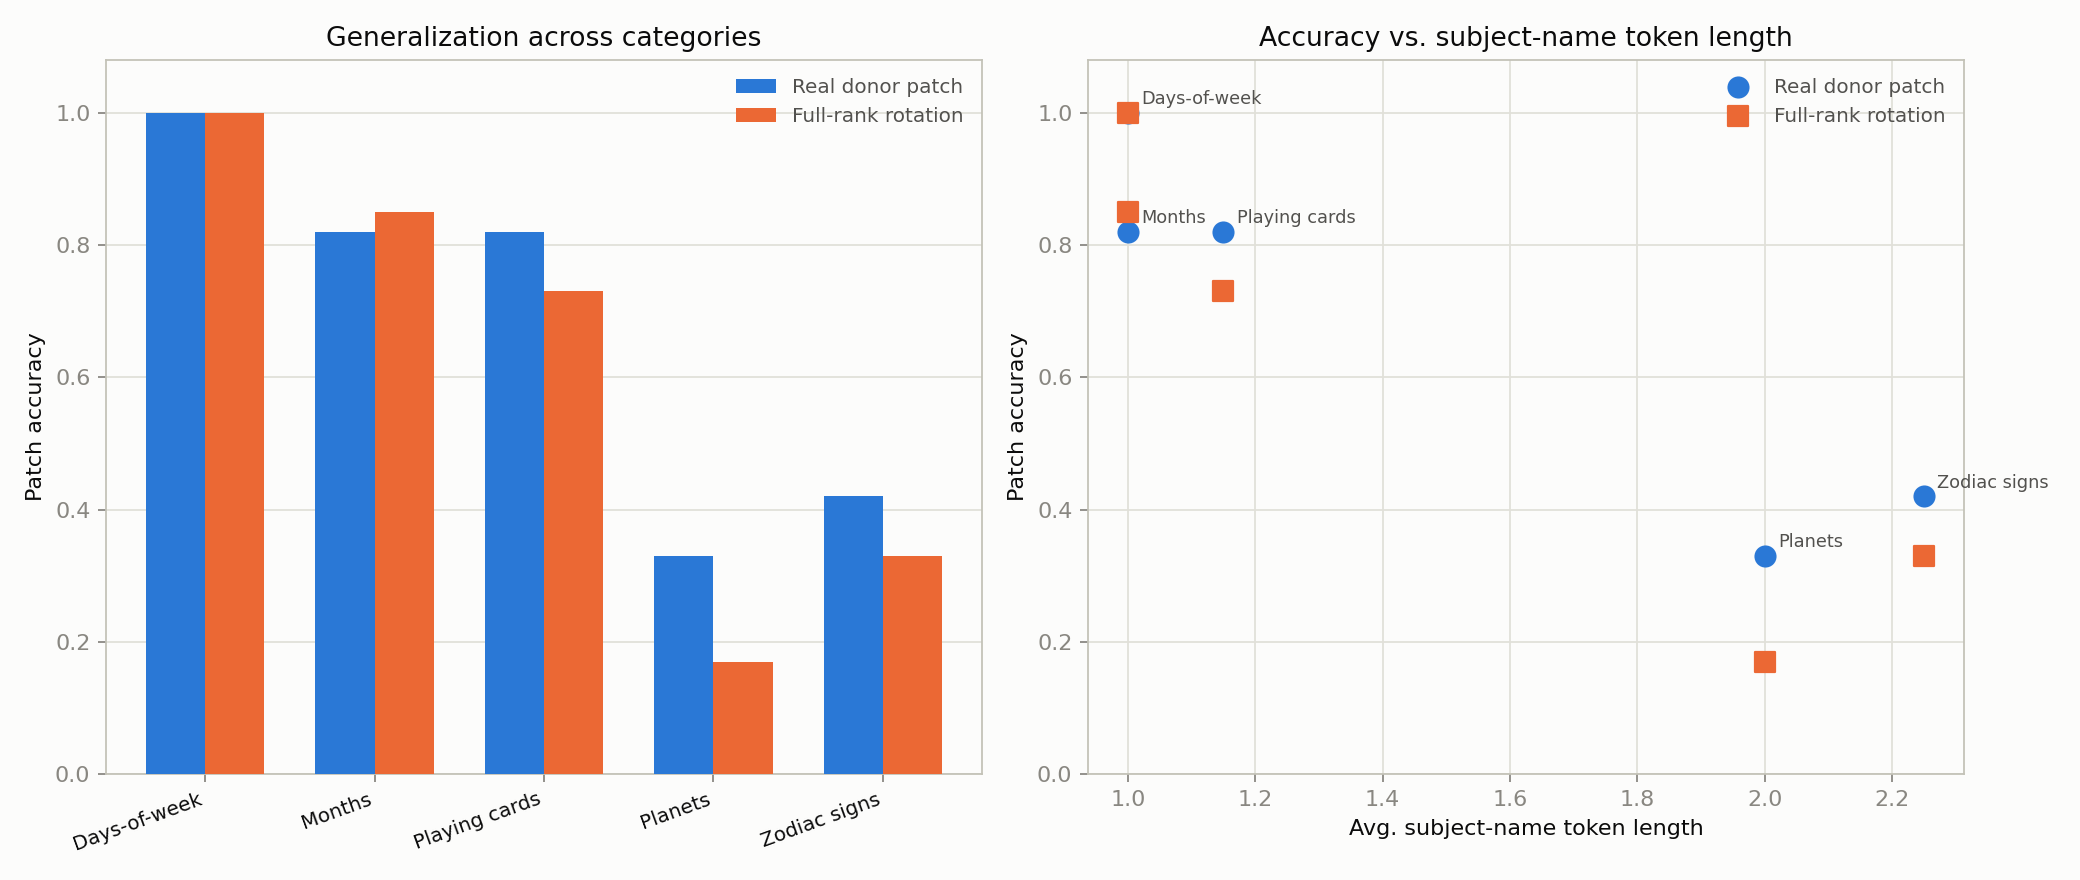
\includegraphics[width=\textwidth]{figures/generalization_summary.png}
  \caption{Left: real-donor vs.\ full-rank-rotation accuracy across all five
  tested categories. Right: the same accuracies plotted against each
  category's average subject-name token length, a near-monotonic
  relationship.}
  \label{fig:generalization}
\end{figure}

The right panel of Figure~\ref{fig:generalization} suggests why: accuracy
tracks average subject-name token length almost monotonically. Days and
months (both exactly 1.00 tokens per name) sit at the top; playing-card
ranks (1.15, since only \emph{Ace} splits into 2 tokens) sit just below;
planets (2.00) and zodiac signs (2.25) sit at the bottom. This is consistent
with, and a natural extension of, the mechanism diagnosed in attempt 1
(\S\ref{sec:causalresult}): patching a single token position leaves any
\emph{other} token of a multi-token subject name unpatched and still visible
to downstream attention. For days and months this was not a limitation,
because the whole subject is exactly one token, there is nothing left
unpatched. For zodiac signs and planets, patching only the final sub-token
of a 2--4-token name necessarily leaves the earlier sub-tokens (e.g.\
\emph{S}, \emph{ag}, \emph{itt} of \emph{Sagittarius}) untouched, giving the
model partial access to the base item's true identity even after patching,
diluting the causal effect in a graded way that scales with how much of the
name is left unpatched. This does not show the underlying representational
code is absent or non-rotational for zodiac signs and planets, only that a
single-token-position intervention captures it less completely the longer
and more fragmented the subject name is.

\section{Discussion}

Six findings, taken together, sketch a coherent picture:

\begin{enumerate}
  \item \textbf{Categorical separation is real, scales with model size, and
        is broader than ``cyclic.''} Calendar/cyclic concepts occupy a
        representational region clearly distinct from quantity, space, and
        relation concepts, confirmed above a randomized-token noise floor in
        the small model, and total graph disconnection in the larger model.
        Scaling to 500 probe tokens across 25 categories
        (\S\ref{sec:scale500result}) refines this: the categories that
        separate cleanly are small, closed, enumerable named sets generally
        (also continents, zodiac signs, playing-card ranks, planets), not
        specifically cyclic or temporal ones, while categories chosen to have
        no expected structure collapse into one undifferentiated region, a
        second negative control that emerged from the data itself.
  \item \textbf{A clean 2D circular manifold did not emerge from bare-word
        probing, in either model.} It partially emerged for months
        (not days) once we switched to in-context arithmetic prompts that
        force the model to actually use the cyclic structure, and to PCA
        instead of a graph Laplacian.
  \item \textbf{Our first causal patching attempt was not a valid test} of
        whether that structure is functionally used by the model, because the
        intervention did not prevent the model from recovering the relevant
        information from elsewhere in the prompt.
  \item \textbf{Our second causal patching attempt is a valid test, and it
        succeeds cleanly.} Patched at the subject-token position, the
        day/month identity is not just correlational structure: overwriting
        it with a donor's representation, at any of a broad, contiguous band
        of early-to-mid layers, causally redirects the model's answer to
        match the donor, with a random-direction control that never once
        succeeds. The effect has a sharp, well-defined depth cutoff rather
        than fading gradually, suggesting a genuine localization of where
        this identity is read out.
  \item \textbf{A clean 2D loop is not the causal code, even where the loop
        is cleanest.} At the exact position and a layer where identity-swap
        patching works almost perfectly, months trace the most visually
        convincing circle in the whole project, and a synthetic vector built
        by rotating within that circle still fails completely, performing
        identically to a deliberately wrong rotation angle. The causally
        necessary code is real (finding \#4) and is not fully captured by
        this 2D projection (finding \#5): two claims that could easily be
        conflated, and are not the same claim.
  \item \textbf{A full-rank rotation generator recovers the effect
        completely.} Fit once across all items via orthogonal Procrustes in
        an $(n{-}1)$-dimensional subspace, a single consistent rotation
        operator $R$, applied to a base item's own vector with no real donor
        data at all, matches or exceeds the real-donor patch's accuracy for
        both categories, while a fractional-power (off-lattice) control
        collapses to near-chance. The geometric hypothesis was too narrowly
        operationalized in finding \#5, not wrong: the code is rotational,
        just not two-dimensional.
  \item \textbf{The rotation mechanism generalizes partially, and the gap is
        explained rather than mysterious.} Playing-card ranks reproduce the
        days/months result closely; zodiac signs and planets do not, and
        the shortfall tracks average subject-name token length almost
        monotonically. Multi-token subject names leave sub-tokens other than
        the patched position unpatched and visible to downstream attention,
        diluting the effect in proportion to how much of the name escapes
        the intervention, the same leakage mechanism that defeated attempt 1,
        now appearing as a matter of degree rather than all-or-nothing.
\end{enumerate}

This is now, on balance, consistent with the prior published result
\cite{engels2024not}, though it took an extra round to get there: that work
used careful in-context templates across many offsets, PCA-based subspace
discovery, and causal patching localized to the subject-token position,
validated with random-direction controls, and reported that the discovered
circular structure was causally used. Our attempt 2 (\S\ref{sec:causalresult})
uses that same causal-tracing recipe and gets a comparably clean result on
the same causal-validity bar. Our attempt 3 (\S\ref{sec:rotationresult}), a
more direct test of the specifically \emph{geometric} claim restricted to 2
dimensions, produced a clean null. Our attempt 4
(\S\ref{sec:highdimresult}), the same geometric test without that
dimensionality restriction, recovers the effect essentially completely. Read
together, the throughline is: the model has \emph{some} causally
load-bearing, swappable code for day/month identity at the subject-token
position (finding \#4); a naive 2-dimensional version of that code, however
visually convincing (Figure~\ref{fig:rotationpca}), is not sufficient to
reproduce the effect on its own (finding \#5); and a single consistent
rotation operator spanning the full space these items occupy is both
necessary and sufficient to reproduce it, with no real donor vector required
(finding \#6). ``The model represents this as a circle'' turns out to be
closer to correct than our attempt 3 suggested, provided ``circle'' is read
as ``a single consistent rotation generator acting on a higher-dimensional
subspace'' rather than ``a 2D loop you can see directly in a PCA scatter
plot.'' Both the positive result and the negative one were necessary to
reach that more precise statement; either alone would have supported a
less accurate conclusion.

\subsection{Limitations}
\begin{itemize}
  \item The probe set (77 tokens) is far smaller than the 500 originally
        envisioned.
  \item Mistral-7B was run in 4-bit quantization to fit an 8GB GPU; this may
        distort fine-grained geometric structure relative to full precision.
  \item The causal-tracing result (\S\ref{sec:causalresult}) establishes that
        the subject-token position causally carries swappable day/month
        identity; it does not by itself establish that this identity is
        encoded as a 2D circle specifically, only that \emph{some} code there
        is causally read and used.
  \item Days-of-week never produced a clean 2D loop in any of the Laplacian,
        PCA, or rotation experiments, even though the causal-tracing result
        for days is just as clean as for months: a real, used representation
        can exist at a position without our chosen 2-component projections
        managing to visualize it as a recognizable shape.
  \item The full-rank rotation generator (\S\ref{sec:highdimresult}) was fit
        with only 6 or 11 components, the maximum available from just 7 or
        12 items. We cannot yet distinguish a genuinely $(n{-}1)$-dimensional
        rotational code from a lower-dimensional one (say, 3 or 4
        dimensions) that PCA with only $n{-}1$ available components happens
        to fit better than 2; testing that would need more distinct items
        per category than the calendar naturally provides (e.g., paraphrases
        or multiple prompt templates per day/month).
  \item The Procrustes fit for the single rotation generator has a
        substantial residual (24--27\%), meaning no single $R$ maps every
        consecutive pair exactly, even though its integer powers still
        reproduce the causal effect almost perfectly; we do not yet have an
        account of why an imperfectly-fit rotation is nonetheless
        behaviorally sufficient.
\end{itemize}

\section{Conclusion}

The underlying research question (whether LLMs represent certain relational
concepts as literal low-dimensional geometry) is a real, current, and
answerable one, but requires more targeted methodology than a generic
similarity-graph Laplacian over isolated words. We found genuine, above-noise
categorical structure (calendar concepts separate cleanly from quantity/space
concepts, more so in a larger model); a visually clean 2D loop for months (not
days) at the subject-token position; a clean, strongly positive causal-tracing
result showing that day/month identity at that position is genuinely
load-bearing for the model's answer, with a sharp and informative
depth-of-localization cutoff; a direct, controlled null result showing that a
synthetic vector built purely from rotating within that same clean 2D loop
carries none of that causal effect; and finally, extending the same rotation
idea to a full-rank subspace instead of just 2 dimensions, a clean positive
result that recovers the effect almost entirely, matching the real-donor
upper bound for both categories while a matched fractional-power control
collapses to chance. Put together: the model has a real, causally necessary,
and genuinely rotational code for day/month identity at this position. A
naive 2-dimensional reading of that code, however visually convincing,
is not the causally sufficient version of it; the causally sufficient
version requires the fuller space these items actually occupy. Both the
positive and negative results were needed to arrive at that more precise
picture, and we would not trust either finding in isolation nearly as much as
we trust them together. Testing the same mechanism on other small closed
sets discovered along the way (zodiac signs, planets, playing-card ranks)
produced neither a clean universal confirmation nor a clean refutation: it
holds up well for playing cards and weakly for zodiac signs and planets, and
that gap is well predicted by how many subword tokens each category's names
occupy, not by anything specific to those categories' content. That, in
turn, sharpens the scope of the entire causal story: what we have evidence
for is a rotational code at a specific token position, and our ability to
detect it with a single-position patch degrades gracefully as the subject
name we are patching stops fitting in that one position.

\appendix
\section{Original planning notes}
\label{app:notes}
The investigation began from a short planning document (\texttt{NOTES.md})
which framed the goal as testing whether ``a continuous, geometric
concept-manifold spontaneously reconstruct[s] itself out of abstract machine
data'' via mutual-information/cosine-similarity graphs and graph Laplacian
diagonalization. All code referenced in this paper is included under
\texttt{code/}, and the raw intermediate data (activation vectors,
similarity graphs, eigenmode projections) is included under \texttt{data/},
at each project phase. The note is reproduced below, verbatim except for
formatting.

\begin{quote}
\small
\textbf{NOTES: The Machine Latent Space Coordinate Reconstruction Challenge}

\textit{Objective.} Bypass verbose machine learning interpretations and
treat an artificial neural network's hidden layer as a discrete,
non-spatial relational substrate. Apply the exact-diagonalisation and graph
Laplacian pipelines developed in the \texttt{universal-emergent-geometry}
repository to test whether a continuous, geometric concept-manifold
spontaneously reconstructs itself out of abstract machine data.

\textit{Architectural framework.} (Raw Token Activations) $\to$ (Compute
Mutual-Information Matrix $I(i,j)$) $\to$ (Diagonalise Graph Laplacian
$\Delta_Q$) $\to$ (Emergent Coordinate System) $\to$ (Causal Activation
Patching)

\textit{Step-by-step execution plan.}
\begin{itemize}
  \item \textbf{Phase 1: Substrate extraction.} Target compact, fully
        open-weight models (e.g.\ Qwen2.5-0.5B or TinyLlama-1.1B). Input a
        structured dataset of 500 semantic tokens spanning hard relational
        categories (linear number sequences, geometric shapes, spatial
        directions, causal relationships). Write a PyTorch activation-hook
        script to intercept the model's forward pass and extract the raw,
        high-dimensional hidden-state activation vectors from the
        mid-point layers (e.g.\ layer 12 of 24) where abstract structural
        relations stabilize.
  \item \textbf{Phase 2: Relational graph construction.} Treat each
        semantic token's activation vector as a state node. Calculate the
        exact cosine similarity or statistical mutual information
        $I(i,j)$ between every node pair to construct a definitive
        $500 \times 500$ relational correlation matrix. Assemble the
        unnormalised graph Laplacian ($\Delta_Q$) directly from this
        relational kernel, completely bypassing any geometric background
        assumptions.
  \item \textbf{Phase 3: Exact-diagonalisation and manifold mapping.}
        Execute a clean numerical exact-diagonalisation of the graph
        Laplacian operator. Plot the lowest-lying non-trivial eigenmodes
        ($\lambda_1, \lambda_2, \lambda_3$) as spatial coordinates. Observe
        whether the low-lying spectrum cleanly reconstructs smooth,
        low-dimensional spatial geometry (circles, lines, or tori) matching
        the intrinsic logic of the input concepts.
  \item \textbf{Phase 4: Causal validation via activation patching.} A
        geometric pattern in the eigenmode plot is only correlational -
        it does not show the model actually \emph{uses} that structure.
        From Phase 3, extract the subspace spanned by the discovered
        eigenmodes (e.g.\ the 2D plane containing a suspected circular
        manifold for a cyclic category like days-of-week or months).
        During a fresh forward pass on a held-out prompt, intercept the
        residual stream at the same extraction layer and directly edit the
        token's activation: project onto the discovered subspace, rotate
        or translate it by a known amount along the recovered coordinate
        (e.g.\ rotate the circle by the angle corresponding to ``+2
        days''), then let the forward pass continue unmodified. If the
        eigenmode coordinates are the model's real internal representation,
        the patched forward pass should shift the output logits/next-token
        prediction in the exact direction predicted by the geometry (e.g.\
        patching ``+2 days'' along the recovered circle should shift
        ``Tuesday'' to ``Thursday''). As a control, repeat the same patch
        using a random direction of matched norm, orthogonal to the
        discovered subspace - this should produce no consistent,
        semantically predicted shift in outputs. Report the
        patched-prediction accuracy across many prompts/categories,
        compared against the random-direction control's accuracy.
\end{itemize}

\textit{Hard constraints and verification checks.}
\begin{itemize}
  \item \textbf{The $g=0$ decoupling control:} randomized or fully shuffled
        token inputs should collapse the graph Laplacian spectrum to a
        flat, featureless noise envelope.
  \item \textbf{Pipeline validation:} token-indexing layouts must not
        silently map trailing token dependencies onto wrong physical
        vector spaces during batch compilation.
  \item \textbf{The causal requirement:} do not claim the geometry is
        ``used'' by the model on representational evidence alone - the
        Phase 4 patching experiment must show patched-direction predictions
        beat the random-direction control before any functional claim is
        made.
\end{itemize}
\end{quote}

\begin{thebibliography}{9}

\bibitem{belkin2003laplacian}
M. Belkin and P. Niyogi.
\textit{Laplacian Eigenmaps for Dimensionality Reduction and Data
Representation.}
Neural Computation, 15(6):1373--1396, 2003.

\bibitem{engels2024not}
J. Engels, I. Liao, E. J. Michaud, W. Gurnee, M. Tegmark.
\textit{Not All Language Model Features Are Linear.}
arXiv:2405.14860, 2024.

\bibitem{meng2022locating}
K. Meng, D. Bau, A. Andonian, Y. Belinkov.
\textit{Locating and Editing Factual Associations in GPT.}
Advances in Neural Information Processing Systems (NeurIPS), 2022.

\end{thebibliography}

\end{document}
